\chapter{Background}
    This chapter introduces the concepts used during the experiments, both within acoustics and machine learning.
    
    %In this chapter, we introduce the context of the work to give the reader an understanding of its importance, and then the concepts used during the experiments both withing acoustics and machine learning.
    
\section{Acoustics}\label{acoustics}
    %When fisheries conduct acoustic surveys of fish, they use \textit{echo sounders} to remotely detect and observe targets in the water. Echo sounders are a special variety of \textit{sonar}, where the acoustic beam is directed vertically downwards from the measuring platform. 
    
    The echo sounder consists of a \textit{transmitter} that produces a burst of electrical energy at some set frequency. Then a \textit{transducer} receives the output from the transmitter and converts it to an acoustic signal that is propagated through the water, which is also called a \textit{ping}. This forms a directional beam akin to the light from a handheld flashlight. Targets in the water \textit{backscatter}/\textit{reflect} parts of the energy back towards the transducer. The transducer detects the backscattered sound or \textit{echo}, and the sound is converted back to electric energy as the received signal and is further amplified. The time when the signal is received determines the range to the target \cite{simmonds2008fisheries}.
    
    Pings are usually represented as columns in a 2-dimensional image, also called an \textit{echogram}, with range along the y-axis and time of ping along the x-axis. The columns represent how the acoustic reflections vary for each ping. Any targets detected in the ping will be visualized as a mark in the echogram, usually with different colors depending on the echo strength. In multi-frequency sonars, individual echograms are produced in parallel for each frequency in use, and this is visualized in figure \ref{echogram_example_fig}. Because the echograms are constructed as $\text{time} \times \text{range}$, the vertical magnitude of a mark indicates the height of the target. At the same time,  the horizontal position illustrates changes in \textit{time} if the echosounder is stationary or in \textit{space} if moving. When moving, the echogram thus represents a vertical cross-section of the water column as the transducer is in motion through the water at constant speed in one direction \cite{simmonds2008fisheries}.
    
    %If the echosounder was stationary, the echogram would be a time-series representation of the same volume. Combined with trawl samples and knowledge of species composition, the mark can be assigned to a specific or group of species.
    
    \begin{figure}[H]
        \centering
            \includesvg[inkscapelatex=false,width=1\textwidth,keepaspectratio]{figures/echogram-echosounder.svg}
        \caption[Echosounder]{Concept of an echosounder: Pings generate echoes from a school of fish and the seabed, and the echoes are displayed in an echogram.}
      	\medskip 
        \label{echogram}
    \end{figure}
    
    \begin{figure}[H]
        \centering
            \includesvg[inkscapelatex=false,width=1\textwidth,keepaspectratio]{figures/acosutic_data.svg}
        \caption[Echosounder]{Example echograms from multiple frequencies.}
      	\medskip 
        \label{echogram_example_fig}
    \end{figure}

%\subsection{Acoustic Propagation and Noise}
    
\subsection{Acoustics and Fish}
    To measure the force of backscattered sound received from a target, the backscattered cross-section $\sigma_{bs}$ or the \gls{ts} is used. They are defined as:
    
%    \begin{equation}
%        \sigma_{bs} = %r^{2}\frac{I_{b}10^{\alpha r/ %10}}{I_{i}},
%    \end{equation}
    
      \begin{equation}        
       \sigma_{bs} = r^{2}\frac{I_{b}}{I_{i}},
   \end{equation}
    

    \begin{equation}
        \textrm{TS} = 10 \log_{10}(\sigma_{bs}),
    \end{equation}
    where $I_{b}$ is sound intensity backscattered from the target, $I_{i}$ is the intensity of the ping at some arbitrary distance (usually 1m), and \textit{r} is the distance away from the transducer($\sigma_{bs}$ in units $m^{2}$). $\sigma_{bs}$ can vary greatly depending on the frequency used, the composition, angle and shape of the target, absorption through sound being converted to heat, and several other factors as described in \citet{simmonds2008fisheries}. 
%$\alpha$ is the acoustic absorption coefficient,

\subsection{The Volume Backscattering Coefficient}
    Individual targets in some sampled volume may be small and plentiful, resulting in their echoes combining and forming a continuous backscattered signal with varying amplitude. Single targets are no longer possible to distinguish, but the signal itself is a measure of the biomass in the water column. This is measured using the \gls{sv}, defined as:
    
    \begin{equation}
        s_{v} = \sum \sigma_{bs} / V_{0},
    \end{equation}
    
    where a sum over all discrete targets returning echoes in the sampled volume ($V_{0}$) is taken. There is a linear relationship between the abundance of fish and \gls{sv} as long as the species or group of species is known. Furthermore, it is important to exclude the bottom echo when fish are being surveyed. As some fish like the sandeel may be found in schools close to the bottom, and if the discrimination of the bottom is poor, there will be large errors in the estimated fish density. For more details on \gls{sv} and bottom detection, see \citet{simmonds2008fisheries}.
    
%    Hei,
%Det finnes en del på dette (se under). Vi bruker 200 kHz når vi finner stimer, men vi %ser at 18KHz og 38 KhZ er viktige for klassifiseringen. 
%
%\citet{sizedependentfreqrespons2009johnsen} - In earlier mentioned annual Norwegian %sandeel surveys the 
%
%\cite{johnsen2017collective} - Bottomconntected schools
%
%\citet{Greenstreet} - 38kHz was adequate but not optimal, with 120kHz as help %discrimination. Sandeels provide a better acoustic return at higher frequencies. 
%
%\citet{pedersen2009relative} - several analyses fish can have species specific reflected %spectrum. backed by. \
%
%\citet{mohammed2006acoustic} - Investegated 18, 38, 120, and 200 kHz. Combinations of sv %can be used to efficiently discriminate between sandeel from herring and mackerel. %Frequency respons instead of relative was better, and more imporant than position and %shape (støtter translation invariance). Some weakness around the use of sv, and better %to use the entire school echo. 
%
%\citet{korneliussen2008proposals} - Multifrequency use can give more information about %acoustic targets. 
%
%\citet{Forland2014Broadbandwidth} - The backscatter from sandeel vary with its %orientation. Causes a behavior where they do not always swim horizontally, slim bodies %,increases the difficulty of interpretating State: Relative low TS because of their lack %of swimmingbladder. backstatter increases with fish size and frequency. Measured the %backscatter of different bodyparts. Many studies have been conducted to find estimates %of sandeel TS at different freqs, but many studies are hard to make use of. %\citet{yasuma2009density} - Back the angle problem, drastic variation in TS by body %length. 
%
%\cite{FREEMAN2004141} - QTC VIEW was used to identify acoustic changes in the properties %of the seabed in the presence of buried sandeels, whilst the EK500 simultaneously %recorded temporal changes in their distribution throughout the water column.
%
%
%OKEIDA SKRIV OM TARGET STRENGTH

%\section{Accoustic Classification of Sandeel (ammodytes marinus)}
%
%https://academic.oup.com/icesjms/article/66/6/1100/694183?login=true 
%- Size-dependent frequency response of sandeel schools
  %  - historically hard to identify because no swim-bladder
  %  - 200kHz for schools, 18 og 38 for individ-classifying
  %  - some work shows:
   %     - some difficulty classify schools og sandeel at 38 and 120kHz
   %     - combinations of Sv at 18, 38, 120, and 200 kHz can effectively identify schools of %sandeel vs. mackerel and herring
   % - goal
   %     - The objective of this study was to identify and exploit differences in frequency %responses to classify sizes of sandeel in schools.
   % - method in works:
   %     - 18, 38, 120, and 200 kHz - further details in paper
   %     - The borders of the schools were delineated in the 200-kHz echogram, because the Sv %from sandeel is strongest and the reverberant noise from gas-bearing phytoplankton is %lowest at this frequency. Catch and multi-f class for identification.
   %     - To compare the frequency responses of each school, the sA measured at i frequencies %(f) were normalized by the mean sA for the four values of f, resulting in proportional %frequency responses [r(f)] -> 10 * log-scaled
   %     - Changes in fish behaviour could change their R(f) values at 120 and 200 kHz, %possibly affecting the classification rate
   %     - In the shallow water characteristic of the sandeel grounds, the sampling width of %the echosounder beam is small compared with the width of the trawl. Therefore, there %is a high probability of a mismatch between trawl catches and acoustic observations %for small schools in proximity to each other
   %     -There was a significant size-dependent difference in the normalized frequency %response of schools comprising small, 1-year-old, and large, 2-year-old 
   %     - proportional frequency responses [R(f)] at 18, 38, 120, and 200 kHz as independent %variables.
%    \begin{itemize}
%        \item ~Deep learning acoustic data
%        \item litt historie kanskje 
%        \item 2021 model, instance segmentation
%        
%        \item X Johnsen autonomous vessels
%        \item Best frequency - 200kHz, and others
%        \item X A review of unmanned vehicles for the detection and monitoring of marine %fauna

         %Our approach is based on a subfield withing \textit{machine learning} called \textit{deep learning} which will be detailed in the next section. 

    % hvordan IMR gjør det idag, og hvorfro vi trenger videre utvikling av metoder. 

%\subsection{Large Scale Survey
%System}




\section{Machine Learning} \label{Machine Learning}
    Machine learning can be split into four parts; the \textit{algorithm}, \textit{empirical data}, a \textit{task}, and a \textit{performance} measure \cite{Goodfellow-et-al-2016}. A machine learning algorithm is designed to increase performance on a task, given data. During this process, also called \textit{training}, the algorithm is said to be \textit{learning} by fitting a \textit{model} to the data. The two machine learning approaches used in this thesis are supervised learning and unsupervised\cite{Goodfellow-et-al-2016}. 
    %Goodfellow-et-al-2016_ML
    %Goodfellow-et-al-2016_E
    
    \subsection{Algorithm approaches} \label{Algorithm types}
        \subsection{Supervised learning}
            Supervised learning  algorithms are defined by the data consisting of an input and the desired output \cite{Goodfellow-et-al-2016}. The algorithm will have to learn a function, mapping from input to correct output. In classification problems, the output would be a class label, for example, classifying pictures of cats from other animals. While in regression problems, the output is a value within a numerical range. For example, predicting the height of a person.
            %Goodfellow-et-al-2016_E
            
        \subsection{Unsupervised Learning}
            Unlike supervised learning, unsupervised learning algorithms only receive the input and learn properties contained in the data \cite{Goodfellow-et-al-2016}. A practical example is clustering, where the samples in a dataset are divided into clusters of similar properties. 
                %Goodfellow-et-al-2016_E
        %\subsection{Reinforcement Learning}
            %In reinforcement learning \cite{Goodfellow-et-al-2016_E}, the algorithm does not learn from a given dataset, but acts in an environment. In some cases, this is a feedback loop, giving either a positive or negative reward for performing certain actions. Examples can be seen in the AlphaZero software that beat professional chess players\cite{silver2017mastering}.
    
    \subsection{Data and Features}
    The quality of the input data to a machine learning algorithm will likely affect its performance \cite{najafabadi2015deep}. Data must be gathered, integrated, cleaned of errors, preprocessed, and features often extracted before being used in learning. Hence, time allocated to prepare and increase the data quality can exceed the time spent learning. The process of extracting features is often referred to as \textit{feature engineering}. It constructs a representation of the data with the most important factors to solve the task. This is often domain specialized and usually requires human involvement. In the next section, \gls{ann} are introduced, which is one avenue within machine learning that can automate the extraction of complicated feature representations during learning.


\section{Artificial Neural Networks} \label{neural networks}
    This section introduces the basic components of an \gls{ann} and how these are combined to create a \textit{deep learning} network/ model. 

    \subsection{Perceptron} \label{perceptron}
        The \gls{ann}s fundamental building block is called an artificial \textit{neuron} or \textit{perceptron}. It consists of a linear regression with the tunable parameters $w$ and $b$ inside a non-linear activation function, explained later in section \ref{activation function}. The perceptron is formulated in the following way \cite{razavi2021deep_exp_per}:
            \begin{equation} \label{eq_perceptron}
                y = g (\sum_{i=1}^{D}w_ix_i + b)
            \end{equation}
            
        where D is the number dimension of the input space, $x$ is the input vector, $w$ is a set of weights of the same size as $x$, $b$ is the bias, and $g$ is the activation function. The single output value \textit{y}, also called the neurons' \textit{activation}, is a weighted sum of the input and weights plus the bias, transformed by the activation function. The perceptron is illustrated in figure \ref{Perceptron / MLP}.
    
    \subsection{Multi-Layered Perceptron} \label{MLP}
        The neurons presented in section \ref{perceptron} are organized together in layers to form an \gls{ann}, which in turn forms what is called a \gls{mlp} \cite{razavi2021deep_exp_per}. If all neurons in each layer are connected to every neuron in the next layer, they form a type of \gls{ann} called \textit{fully connected} networks. An \gls{mlp} is depicted in figure \ref{Perceptron / MLP}.
        
            \begin{figure}[H]
                \centering
                
                \subfloat[Perceptron/neuron.]{
        	\includesvg[inkscapelatex=false,width=0.4\textwidth,keepaspectratio]{figures/neuron.svg} \label{perceptron fig}}
        	
        	       \subfloat[An \gls{mlp} with four inputs in the input layer(arrows to the left), two hidden layers(\textbf{h}), and three outputs in the output layer($\hat{\textbf{y}}$).]{
        	\includesvg[inkscapelatex=false,width=0.5\textwidth,keepaspectratio]{figures/mlp.svg}\label{mlp fig}}
                %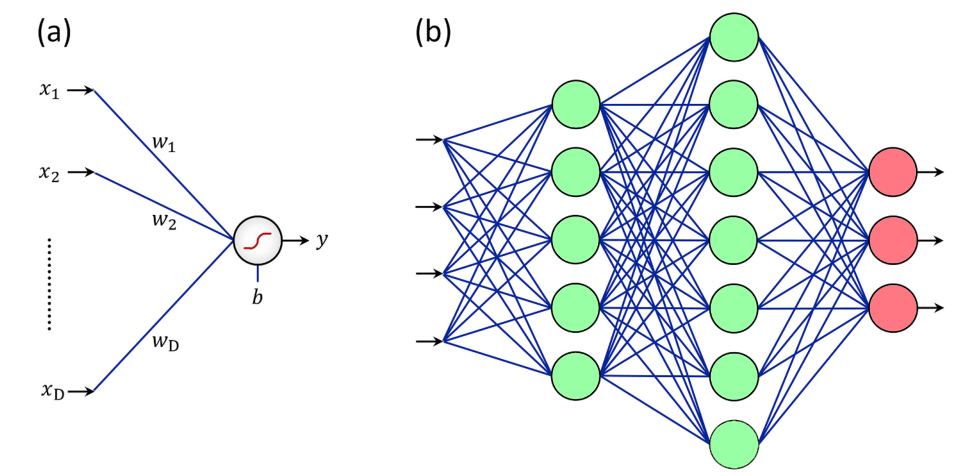
\includegraphics[scale=0.5]{figures/perceptron.png}
                
                \caption[The perceptron and multi-layer perceptron]{Illustration of a single neuron and a fully connected deep learning network of neurons.}
              	\medskip 
                \hspace*{15pt}\hbox{\scriptsize Credit: \citeauthor{razavi2021deep_exp_per} \cite{razavi2021deep_exp_per}}
                \label{Perceptron / MLP}
            \end{figure}
        
        The \textit{architecture} of any \gls{ann} consists of an input layer, a user-defined number of \textit{hidden layers}, and finally, an output layer \cite{razavi2021deep_exp_per}. More hidden layers form a \textit{deeper} network, hence the name \textit{deep learning}. An \gls{mlp} is a type of network called a \textit{feed-forward} \gls{ann} because the data flow from the input to the output layer, and each layer is a function of the previous layer. During training, the weights between every neuron and the bias are optimized in a process that is  further explained in section \ref{training neural networks}. In the MLP depicted in figure \ref{Perceptron / MLP}, different neurons will activate with varying strengths depending on the input, resulting in different outputs. The architecture of the \gls{mlp} in figure \ref{Perceptron / MLP} can be expressed as \cite{Goodfellow-et-al-2016}:
        %Goodfellow-et-al-2016_architecture
        \begin{align}\label{mlp outputlayer eq}
            \textbf{h}^{(1)} &= g^{(1)}(\textbf{W}^{(1)T}\textbf{x} + \textbf{b}^{(1)})\\
            \textbf{h}^{(2)} &= g^{(2)}(\textbf{W}^{(2)T}\textbf{h}^{(1)} + \textbf{b}^{(2)})\\
            \hat{\textbf{y}} &= g^{(3)}(\textbf{W}^{(3)T}\textbf{h}^{(2)} + \textbf{b}^{(3)})
        \end{align}

        
        
%        \begin{equation}
%            \textbf{h}^{(1)} = \sigma^{(1)}(\textbf{W}^{(1)T}\textbf{x} + \textbf{b}^{(1)})
%        \end{equation}
%        \begin{equation}
%            \textbf{h}^{(2)} = \sigma^{(2)}(\textbf{W}^{(2)T}\textbf{h}^{(1)} + %\textbf{b}^{(2)})
%        \end{equation}
%        \begin{equation} \label{mlp outputlayer eq}
%            \hat{\textbf{y}} = \sigma^{(3)}(\textbf{W}^{(3)T}\textbf{h}^{(2)} + %\textbf{b}^{(3)})
%        \end{equation}
        
        where for each layer \textbf{h} is a vector of activations, \textbf{W} is a matrix of weights, \textbf{b} is a  vector of \textbf{biases}, $g$ is an activation function applied element-wise, and $\hat{\textbf{y}}$ is a vector of outputs. %The activation function $\sigma$ can also vary from layer to layer.
        
        
    \subsection{Activation Function} \label{activation function}
    %Goodfellow-et-al-2016_out_activation
        The activation function enables \gls{ann}s to learn non-linear features \cite{razavi2021deep_exp_per}. It is needed because a network consisting of only linear layers will be the same as a single linear layer. Hence, it won't be able to capture non-linearities in the data, and therefore an activation function is required in the hidden layers. Some activation functions can also be applied to the network's output to solve the task the network is set to perform and must be suited for the task at hand \cite{Goodfellow-et-al-2016}. The activation function commonly used in the hidden layers is ReLU, which stands for \textit{rectified linear unit} \cite{sharma2019new_activation_func}. ReLU takes a real number as input and outputs this number if it is above zero,  otherwise, it will output zero. Letting $g$ denote the activation function, and $x$ the input, the ReLU activation function can be formulated as follows:
            \begin{equation} \label{relu_eq}
                g(x) = max(0,x)
            \end{equation}
        ReLU is also visualized in figure \ref{activation_fig}. ReLU activate some neurons to propagate their input while preventing others from doing so. This can result in greater efficiency and faster training, as not all neurons are active, further detailed in \citeauthor{sharma2019new_activation_func} \cite{sharma2019new_activation_func}. 
        
        Another activation function is the logistic sigmoid that transforms all input values to values in the range [0…1] \cite{sharma2019new_activation_func}. It could be applied to the output layer to solve binary classification problems, as the values can be treated as probabilities. The formula for logistic sigmoid is:
            \begin{equation} \label{sigmoid_eq}
                g(x) = \dfrac{1}{1 + e^{-x}} 
            \end{equation}
            
            \begin{figure}[H]
                \centering
                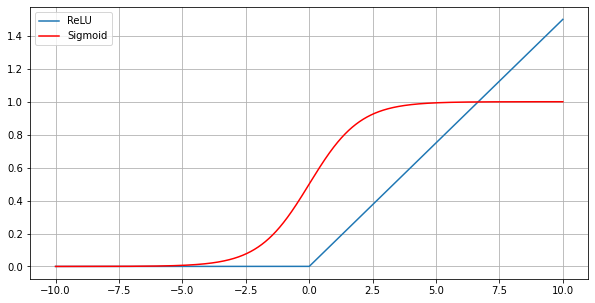
\includegraphics[scale=0.5]{figures/activation.png}
                \caption[ReLu and sigmoid]{A ReLU function (blue) and a sigmoid function (red)}.
              	\medskip 
                \label{activation_fig}
            \end{figure}

    \subsubsection{The Softmax Function}
        The \textit{softmax} can be viewed as a multivariate version of the logistic sigmoid activation function, which allows the softmax to be applied to problems containing multiple classes \cite{sharma2019new_activation_func}. For all data points, it calculates the probability of every class and can be expressed as:
        \begin{equation}
            g(\textbf{x})_{j} = \dfrac{e^{x_{j}}}{\sum^{K}_{k=1}e^{x_{k}}} \textrm{ for j = 1,...,K.}
        \end{equation}
        
        where K is the number of classes, and the output summarizes to 1 over all classes. For a network solving multiclass classification, the output layer will have size equal to K. This corresponds to 3 classes in figure \ref{Perceptron / MLP}. The \textit{softmax} would then be used as the last transformation (\textit{$g^{(3)}$ in equation \ref{mlp outputlayer eq}}) and output the probability of an input belonging to each of the three classes.
        
\subsection{Convolutional Neural Network} \label{cnn}
    The \gls{cnn} is a type of \gls{ann}s primarily used in machine learning tasks concerning images \cite{o2015introduction_convolutions}. One of the reasons why the \gls{cnn} emerged was because images input to a regular \gls{ann} produces a large number of learnable parameters. For example, a low-resolution image with $512\times512$ pixels passed to an hidden layer containing only one neuron would have $1\times512\times512 = 262144$ weights alone.  To solve this issue and have fewer learnable parameters, the modern \gls{cnn} is built around three main components \cite{o2015introduction_convolutions}; a \textit{convolutional layer}, a \textit{pooling layer}, and a \textit{fully-connected layer}. An example \gls{cnn} is illustrated in figure \ref{convolutional_neural_network_fig}, and each main component will be explained later in this section.

    \begin{figure}[H]
        \centering
                        \includesvg[inkscapelatex=false,width=0.95\textwidth,keepaspectratio]{figures/conv_net.svg}
        \caption[Convolutional neural network example]{Illustrations of the main components in a \gls{cnn}.}
      	\medskip 
        \label{convolutional_neural_network_fig}
    \end{figure}

%The \textit{flatten} operation is applied here to make the output from the pooling layer compatible with the fully connected layer of regular neurons.


    \subsubsection{Convolutional Layer}
    
    
     \citeauthor{o2015introduction_convolutions} \cite{o2015introduction_convolutions} describe the convolutional layer as consisting of many learnable multidimensional weight matrices that slide over the input. We will refer to such a matrix as a \textit{kernel}. The kernel's height and width are parameters defined by the user, but the depth will always be equal to the number of channels in the input. This results in kernels being described only by $height \times width$. The kernel slides over the input, and is applied to different locations of the input, also called the current \textit{receptive field}. A single scalar value is computed when applied, which is the weighted sum of the kernel's weights and the corresponding values in the receptive field. If we have a 2-dimensional image $I(i,j)$ as input, a convolutional operation is expressed as \cite{Goodfellow-et-al-2016}:
     %Goodfellow-et-al-2016_convolution
        \begin{equation}
            (I*K)(i,j) = \sum_{height}\sum_{width}I(i-height,j-width)K(height,width)
        \end{equation}
     
     where $*$ is the convolutional operation, \textit{I(i,j)} is the image pixel at \textit{(i,j)}, and \textit{K} is the kernel.
     
    The output scalar value from the convolutional operation is usually fed through non-linear activation functions like ReLU and then called the \textit{activation}. The sliding operation is based on a value called \textit{stride}, which is the number of horizontal positions to move the kernel in the input between each calculation. Suppose we started from the left, and it is impossible to move horizontally to the right and still fit the kernel inside the input. In this case, the kernel will, if possible, move rows down vertically equal to the stride and then continue horizontally, starting afresh from the left. After sliding over the entire input, a complete 2-dimensional \textit{activation map}, also called a \textit{feature map}, has been created, one such map for each kernel applied. The idea is that each applied kernel will learn to identify different features in the input. An example of a horizontal edge detector can be seen in figure \ref{convolutional_fig} \cite{o2015introduction_convolutions}. 
    \begin{figure}[H]
        \centering
                \includesvg[inkscapelatex=false,width=1\textwidth,keepaspectratio]{figures/convolutions.svg}
        \caption[Horizontal edge detector example]{Illustration of a \textit{valid} (detailed later in this section) convolutional operation. The kernel is applied repeatedly across the input. The input size is 6×6, kernel size is 3×3, and stride 1, resulting in overlapping operations and output size being 4×4. The figures to the right show the input, kernel, and output(activation) as color gradings, where the color gets darker if the values are low. This example is a horizontal edge detector, and the result is large values in the activation map along the border between the values of 0 and 10 in the input, which could have been colors in a picture.}
      	\medskip 
        \label{convolutional_fig}
    \end{figure}
    
    The receptive field will start as small regions, but as we apply additional convolutional layers, it will have access to increasing context in regard to the input \cite{Goodfellow-et-al-2016}. This is illustrated in figure \ref{receptive_field_fig}, and kernels in early layers learn to identify simple features while later combining these to identify complex features. The kernels utilizes \textit{parameter sharing}, as the same weights are repeatedly used across the input. Furthermore, the kernels are often smaller than the input, resulting in \textit{sparse connections} as opposed to fully connected networks. The parameter sharing results in the \gls{cnn} having another useful attribute called \textit{equivariance}, which means that if the input changes, the output changes in the same way.
    \begin{figure}[H]
        \centering
        \includesvg[inkscapelatex=false,width=0.9\textwidth,keepaspectratio]{figures/receptive_field_clown.svg}
        
        \caption[Receptive field]{The activation maps from two convolutional layers with 3×3 kernels and stride 1. The first convolution's receptive field is marked as red. On its activation map, a new convolutional layer is applied. Its first receptive field is outlined in green, which translates to a larger area in the input.}
      	\medskip 
        \hspace*{15pt}\hbox{\scriptsize Credit: Original image by Nick Hobgood \cite{clownfish_image}, used as input picture above (Edited with colored grid).}
        \label{receptive_field_fig}
    \end{figure}
   The application of \gls{cnn}s on acoustic data can be motivated by the echograms being similar to regular images, but the RGB color channels being replaced with the different frequency channels measured. However, the same object will be represented differently in echograms at varying ranges from the transducer, possibly similar to objects of another class \cite{simmonds2008fisheries}. This likely increases the complexity of target classification in acoustic data, as benefits of equivariance is not as applicable.
 
    %which is that the location of the feature in the input is not relevant to a convolutional neural network. %Combined, this creates a layer able to detect features in an input with fewer learnable parameters than a normal \gls{ann}. 
    


    %The complete \textit{convolutional operation} performed by a convolutional layer consists of applying this kernel to the entire input. Producing activations for different regions of the input. This reduces the dimension of the input to a 2D activation output, but you may apply several kernels to increase the channels, as each will create a new 2D channel in the activations. A convolutional operation is often followed up with an element wise nonlinear activation function to its activations, like a ReLu. The kernels will through training learn to detect different features in the input, and so in a \gls{cnn} the first layers will often detect simple features like edges. Later layers will then detect more complex features like cars and houses, combining the activations from different earlier layers. The last layer consists of a \textit{fully connected} layer of regular neurons to determine the output, but implementations of networks with only convolutional operations exists like U-Net which will be described\cite{unet_ronneberger2015} in section \ref{unet} utilizing 1x1 convolutions. A more detailed example can be found in figure \ref{convolutional_fig} which looks at how a convolution with a horizontal edge detecting kernel is applied to a single channel or an equivalent 2D input. 
    
    Reductions in the spatial size will normally occur with the convolutional operation described in this section, and such operations are called \textit{valid convolutions} \cite{o2015introduction_convolutions}. By applying padding with zeros around the input, we can retain the dimensions of the input. The effect is that more convolutional operations fit in the new padded input, hence an equal output size. This is called the \textit{same convolution}, illustrated in figure \ref{same_convolutional_fig}.
    
    \begin{figure}[H]
        \centering
        \includesvg[inkscapelatex=false,width=0.9\textwidth,keepaspectratio]{figures/same_convolutions.svg}
        \caption[Same convolution example]{Illustration of the \textit{same} convolutional operation. The input size is 3×3, but after padding with zeros, the size is 5×5, kernel size is 3×3, and stride is 1. This results in an activation map size of 3×3, conserving the input size.}
      	\medskip 
        \label{same_convolutional_fig}
    \end{figure}
    

    
\subsubsection{The Max Pool Layer}

    \begin{figure}[H]
        \centering
                \includesvg[inkscapelatex=false,width=0.8\textwidth,keepaspectratio]{figures/maxpool.svg}
        \caption[The max pool operation]{Illustrates the max pool operation with size 2×2 and stride 2.}
      	\medskip 
        \label{maxpool_fig}
    \end{figure}
    The max pool layer reduces the \textit{height} and \textit{width} of its input \cite{o2015introduction_convolutions}. Like a convolutional operation, the max pool looks at an input region but instead applies a \textit{max} operation. The pooling kernel size is given in $height \times width$ and is applied individually to each channel of the input. This reduces the height and width but preserves the number of channels. The most common max pool layer is a 2×2 with a stride 2. Alone, the max pool has no learnable parameters and is applied to decrease the computational complexity of the \gls{cnn}.


\subsubsection{Fully Connected Layer}
    \begin{figure}[H]
        \centering
        \includesvg[inkscapelatex=false,width=0.95\textwidth,keepaspectratio]{figures/1x1.svg}
        %\includesvg[inkscapelatex=false,scale=0.3,keepaspectratio]{figures/Bilde1.svg}
        \caption[1×1 convolution]{Illustration of the 1×1 convolution with stride 1. Yellow cells demonstrate the application of a 1×1 kernel along all channels of the input, producing one activation in the output. }
      	\medskip 
        \label{1x1_fig}
    \end{figure}
    \citeauthor{lin2013network_in_network_1x1} \cite{lin2013network_in_network_1x1} proposed the convolutional layer with kernel size 1×1 and stride 1, followed by an activation function. The 1×1 layer will take the weighted sum along a 1×1 slice through all channels of the input, as illustrated in figure \ref{1x1_fig}. This is equivalent to applying a fully connected layer to the same values. As this preserves the \textit{resolution}, it can be used to alter the depth of the output feature maps by specifying the desired number of kernels, while also introducing non-linearity. In figure \ref{1x1_fig}, we have only one kernel, but if two were applied instead, the output feature map would have a depth of two. In this work, it is used mainly to map high dimensional feature maps to the desired number of classes.
    
    
    %This is equivalent to the regular hidden layer shown earlier in figure \ref{Perceptron / MLP}, but for one pixel across the channels of the input.

\subsubsection{Transposed Convolutions}
    \begin{figure}[H]
        \centering
        \includesvg[inkscapelatex=false,width=0.95\textwidth,keepaspectratio]{figures/transpose_conv.svg}
        
        
        \caption[Transposed convolution]{Illustration of the transposed convolution operation with kernel size 2×2 and stride 1. The green color shows one of the intermediate computations. The center value of each crop is outlined to illustrate the summation step as these overlap.}
      	\medskip 
        \label{transposed_conv_fig}
    \end{figure}
    A transposed convolution is an operation taking an input, and with a kernel similar to that described in \ref{cnn}, but now instead map the input to a higher resolution \cite{dumoulin2016guide_transposed_convolution}. In example figure \ref{transposed_conv_fig}, a 2-dimensional 2×2 input is fed to a transposed convolutional layer with kernel size 2×2. The whole kernel is multiplied element-wise with the input and proceeds to produce values in a temporary matrix initialized with zeros, denoted by empty cells in the figure. We do not use the temporary values in practice, but they are used here to illustrate the intermediate computations. The calculated values in the temporary matrix are situated correctly relative to the input. These temporary matrices are then summed over, producing the output. This operation is repeated for all channels, retaining the depth of the input. 
            


\subsubsection{Segmentation}
    \begin{figure}[H]
        \centering
        \includesvg[inkscapelatex=false,width=1\textwidth,keepaspectratio]{figures/segmentation_clown.svg}
        \caption[Difference between semantic and instance segmentation]{Illustration of the difference between semantic and instance segmentation.}
      	\medskip 
        \hspace*{15pt}\hbox{\scriptsize Credit: Original image (\textit{Input picture above}) by Nick Hobgood\cite{clownfish_image}}
        \label{segmentation_fig}
    \end{figure}

    Segmentation is a task where the objective is to assign one or several classification masks to the input, usually a picture \cite{He_2017_ICCV_segmentation}. This is further split into two different categories: \textit{semantic} and \textit{instance} segmentation. In semantic segmentation, we assign each pixel in the input to predefined classes. The output would have the same resolution as  the input but with channels equal to the number of classes. A softmax would then be calculated for each pixel across the depth, and the pixel would be assigned to the class with the highest probability. Hence, producing a mask for each class. In instance segmentation, we increase the complexity by applying semantic segmentation while simultaneously assigning a bounding box to each object, as visualized in figure \ref{segmentation_fig}.
    
\section{Training Neural Networks} \label{training neural networks}
    This section will describe the main concepts behind how neural networks are trained to perform on various tasks. 

\subsection{Forward-Propagation and The Loss Function}
    %    A \gls{ann} can be  described as an unknown function \textit{\^{f}} that maps an input \textbf{x} to an output \textbf{y}\cite{Goodfellow-et-al-2016_NN}. 

    The objective of an \gls{ann} is to approximate some optimal function \textit{f}, and in this thesis, we focus on classifiers, $\textbf{y} = f(\textbf{x})$, which maps an input \textbf{x} to an output category \textbf{y}. The \gls{ann} approximates this function by defining a mapping, $\textbf{\^{y}} = \hat{f}(\textbf{x},\theta)$, and learns the values of the parameters \textit{$\theta$} (weights and biases) through training using examples. In supervised tasks, the labels instruct the output layer exactly how to perform given the input data. However, the data does not inform the individual \textit{hidden layers} how to behave to produce this desired output. When the data flow through the network using the parameters $\theta$, it produces outputs \textbf{\^{y}}, called the \textit{forward-propagation step}. How the parameters are initialized can heavily affect the training process, and different strategies are further described in \citet{Goodfellow-et-al-2016}. Using a \textit{loss function} to compare the true \textbf{y} values to the estimated values \textbf{\^{y}}, we measure the network's \textit{error}, also called \textit{loss}. The network uses this loss to then alter $\theta$ to best approximate \textit{f}, which will be explained later in section \ref{backpropagation}. In classification tasks, the network is trained to output the probability of each class given an input \cite{ho2019real_weighted_cross_entropy}. We can use a loss function called \textit{weighted cross entropy} to train such a model. This function outputs a loss based on the probabilities, weights classification of certain classes differently, and is often used when dealing with data containing class imbalance as more weight can be applied to the minority class. Expressed as:
    %Goodfellow-et-al-2016_param_init
        \begin{equation} \label{cross_entropy}
            loss(x,y) = - \sum^{n}_{i=1} w_{y_{i}}y_{i}\log(\hat{y_{i}}), \quad \hat{y_{i}} = \hat{f}(x_i,\theta)
        \end{equation}
    
    where \textit{n} is the number of classes, $y_{i}$ is 1 if the $i^{th}$ class is true (\textit{else 0}), $\hat{y_{i}}$ is the output from the softmax for the $i^{th}$ class, and $w_{y_{i}}$ is the weight of the class to which $y_{i}$ belongs. More examples of loss functions can be viewed in \citeauthor{mishra2017deep} \cite{mishra2017deep}.
    


\subsection{Mini-batch Stochastic Gradient Descent} \label{batch learning}
        \begin{quote}
        "\textit{A recurring problem in machine learning is that large training sets are necessary for good generalization, but large training sets are also more computationally
        expensive."} - (\citeauthor{Goodfellow-et-al-2016}\citeyear{Goodfellow-et-al-2016}, page 152)
    \end{quote}
    %Goodfellow-et-al-2016_SGD
    
    Calculating the total loss of the whole dataset is often unfeasible, and depending on the hardware, this could lead to a crash or slow learning due to
    heavy memory demands. A solution is to sample a set of examples, called a \textit{mini-batch}, from the entire dataset, with the intent to approximately estimate
    the true loss using this smaller fraction of the dataset. Then we update the parameters of our network based on this and repeat on a new mini-batch. This is called mini-batch \textit{\gls{sgd}}, a common \textit{optimization} algorithm \cite{Goodfellow-et-al-2016}. The size of this mini-batch can vary from one example (\textit{also called true \gls{sgd}}) to hundreds, and the size chosen can heavily affect training. When we have run this process on all the data, we say that an \textit{epoch} has passed \cite{wilson2001need_learning_rate}.
    %Goodfellow-et-al-2016_SGD
    
    
    
    %The problem, described in the quote above, arises when we have a large dataset, and we would calculate the loss values of all samples before updating the parameters in our network\cite{Goodfellow-et-al-2016_SGD}. Depending on the hardware, this could lead to a crash or slow learning due to heavy memory demands. A solution is then to sample examples from the entire dataset with a uniform distribution, hence forming a \textit{mini-batch}, with the intent to approximately estimate the true \textit{loss} using this smaller fraction of the dataset. We can then update the parameters of our network based on this and repeat on a new batch. When we have run this process on all the data, we say that an \textit{epoch} has passed. . This algorithm is called \textit{\gls{sgd}}\cite{Goodfellow-et-al-2016_SGD}, which utilizes this minibatch form of training, and is used in this thesis. \gls{sgd} optimizes the parameters of the network by minimizing the loss\cite{pmlr-v37-ioffe15_batch_norm}:
    
        %\begin{equation} \label{batch_learning_eq}
            %\theta = \arg \min_{\theta}\dfrac{1}{N} \sum^{N}_{i=1} loss (x_{i},\theta)
        %\end{equation}
    
    %where $\theta$ is the set of parameters to be optimized, $x_{1..N}$ is the training data, and $x_{1..m}$ is a minibatch of the training data. \gls{sgd} is what is called an \textit{optimization} algorithm.
    
    
\subsection{Back-Propagation and Gradient-based Learning}\label{backpropagation}
    To update the network parameters, we use the loss from a mini-batch and iteratively step back through the layers in a process called \textit{back-propagation} \cite{rumelhart1986learning_backprop}. In each step, we calculate the gradient of the loss functions with respect to the parameters of the current layer by using the chain rule. This is to determine how changes to each parameter will affect the \textit{loss}. Using the gradient, \gls{sgd} performs \textit{gradient descent} \cite{Goodfellow-et-al-2016} by updating all parameters in the opposite direction of the gradient to reduce the loss. In what magnitude a parameter is adjusted by the optimizing algorithm is determined by the \textit{learning rate}, usually a value between 0 and 1. The parameter update is expressed as \cite{pmlr-v37-ioffe15_batch_norm}:
    %Goodfellow-et-al-2016_gradient_descent
    \begin{equation}
    \theta^{(j)} \leftarrow \theta^{(j)} - \eta \dfrac{1}{m}\sum_{i=1}^{m} \dfrac{\partial loss (x_i,y_i)}{\partial \theta^{(j)}}
    \end{equation}
    
    where $\theta$ is the parameters of the network, \textit{m} is the mini-batch size, $\eta$ is the learning rate, and \textit{j} is the layer. In figure \ref{learning_rates} an example loss function is illustrated with one global \textit{loss} minima and different learning rates applied with \gls{sgd}. Low learning rate values usually have a long training time and may cause the \gls{sgd} to converge to a local minima instead of the global \cite{farsal2018deep}. However, too high values can overshoot the global minima and diverge. Both can be prevented by applying a method to adapt the learning rate to the \textit{topography} of the loss function. This thesis applied \textit{momentum}, which only acts as a \textit{velocity} to the update step. The \textit{velocity} is based on past steps, and the update will step in the \textit{velocities'} direction, not the current \textit{gradient}. More detail on \textit{momentum} can be found in \citeauthor{pmlr-v28-sutskever13} \cite{pmlr-v28-sutskever13}.
    
    \begin{figure}[H]
        \centering

        \includesvg[inkscapelatex=false,width=1.0\textwidth,keepaspectratio]{figures/learning_rates.svg}
        \caption[Learning rates]{Three different applications of \gls{sgd} on a loss function. Each arrow is an imagined learning step taken by the algorithm for; (a) low learning rate, (b) high learning rate, and (c) momentum.}
      	\medskip 
        \label{learning_rates}
    \end{figure}

    In summary, the entire training process using \gls{sgd} can be described as the following algorithm \cite{farsal2018deep}:
    
    \begin{longtable}{lllllll} \label{sgd algorithm}\\
    \hline
    \multicolumn{7}{l}{Mini-batch SGD one epoch}                                                              \\ \hline
    \endfirsthead
    %
    \endhead
    %
    \hline
    \endfoot
    %
    \endlastfoot
    %
    \multicolumn{7}{l}{Loop:}                                                                       \\
    1.   & \multicolumn{6}{l}{Sample a mini-batch of data.}                                                \\
    2.   & \multicolumn{6}{l}{Forward propagate the mini-batch through the network and compute the loss.} \\
    3.   & \multicolumn{6}{l}{Back propagate to calculate the gradients.}                            \\
    4.   & \multicolumn{6}{l}{Update the parameters based on the gradients.}                         \\ \hline
    \end{longtable}
    
    

%\subsection{Vanishing and exploding gradient} \label{}
    %By repeatedly applying forward-propagation, back-propagation and some optimizing algorithm on new examples as stated by \citeauthor{Goodfellow-et-al-2016_NN}, you train a network to approximate the optimal function \textit{f}.
\section{Model Evaluation}
    To evaluate a machine learning algorithm, we need a performance measure. First, the \textit{performance metric} itself will be described, followed by a technique applied to make unbiased measures of the model by leaving out parts of the data. Finally, two central challenges that appear in machine learning.
    
    \subsection{Performance Metrics} \label{f1_score}
        This section describes the performance metrics used in this thesis. Consider a binary classification system that classifies samples into either the \textit{positive} or \textit{negative} class. Predictions by the classifier can thus be sorted into the following four categories \cite{powers2020evaluation_f1_recall_precision}:
        
        \begin{itemize}
            \item \textbf{True positive (TP):} A correct classification of a positive example.
            \item \textbf{True negative (TN):} A correct classification of a negative example.
            \item \textbf{False positive (FP):} A negative example incorrectly classified as positive
            \item \textbf{False negative (FN):} A positive example incorrectly classified as negative.
            \end{itemize}
        
        We can now calculate the performance of the classifier from these values, and the simplest is accuracy \cite{powers2020evaluation_f1_recall_precision}:
        
        \begin{equation}
            accuracy = \dfrac{\textrm{\textit{correct predictions}}}{\textrm{\textit{total number of predictions}}} = \dfrac{TP+TN}{TP+TN+FP+FN} 
        \end{equation}
        
        This metric does not handle class imbalance well, as it is equivalent to calculating the percentage of correct predictions \cite{powers2020evaluation_f1_recall_precision}. An example is that if 95\% of the data belongs to one class, then always predicting this class will give us an accuracy of 95\%.
        
        We calculate two new metrics to better deal with class imbalance:  \textit{precision} and \textit{recall} \cite{powers2020evaluation_f1_recall_precision}. Precision is the percentage of positive predictions made by the model that are correct. Recall is the percentage of all positive samples the model managed to classify correctly.
        
        \begin{equation}
            \textrm{\textit{precision}} = \dfrac{TP}{TP+FP}
        \end{equation}
        
        \begin{equation}
            \textrm{\textit{recall}} = \dfrac{TP}{TP+FN}
        \end{equation}
        
        Then, by using precision and recall, we calculate the \textit{F1-score} \cite{powers2020evaluation_f1_recall_precision}. It combines these metrics and is designed to work well on imbalanced data. The F1-score formula: %There are of course many other performance metrics, but this section will be limited to describing those used in the thesis. 
        
        \begin{equation}
            \textrm{\textit{F1-score}} = 2 \cdot \dfrac{\textrm{\textit{precision}} \cdot \textrm{\textit{recall}}}{\textrm{\textit{precision}} + \textrm{\textit{recall}}}
        \end{equation}
        
        
        
    \subsection{Train-Validation-Test Split}
        When a machine learning model is learning, the goal is to achieve the lowest \textit{generalization error}. This means to not only perform well on data seen during training, but also on new unseen data. To measure this error, it is normal to split our data into three parts: the \textit{training}, \textit{validation}, and \textit{test} dataset, and we measure some error or metric on each. As the name suggests, the training data is used during the training process of the model. The validation dataset is extracted from the training dataset and gives an unbiased estimate of the models' performance and can be used to guide the training process. The last mentioned could be to select the best model from a selection of many. Finally, the test dataset is used to get an unbiased estimate of the final model's \textit{generalization error} \cite{Goodfellow-et-al-2016}.
        %Goodfellow-et-al-2016_generalization
        %Goodfellow-et-al-2016_train_val_test_split
    
    \subsection{Overfitting Vs. Underfitting}
        A model's performance depends on the difference between its \textit{training} and \textit{test} error. \textit{Underfitting} happens when a model fails to achieve a low training error, while \textit{overfitting} happens when the training error is significantly lower than the test error. To manipulate this behavior, we adjust the model's \textit{capacity}. Capacity represents the variety of functions the model can learn, and by adjusting it, one can increase and decrease the likelihood of underfitting and overfitting. The capacity can be controlled by, for example, changing the number of layers in a neural network, and further details can be seen in \citeauthor{Goodfellow-et-al-2016} \cite{Goodfellow-et-al-2016}. Low \textit{capacity} means that the model may fail to capture patterns in the data. High \textit{capacity} translates to adjusting to the training data to such an extent that the model performance may be worse when given unseen test data. The optimal solution, depicted in the center plot of figure \ref{over/under fit fig}, is to have a model with a balanced capacity that is as close to the true function as possible \cite{Goodfellow-et-al-2016}. 
        
       % \citeauthor{Goodfellow-et-al-2016}\cite{Goodfellow-et-al-2016}
        
        \begin{figure}[H]
            \centering
            %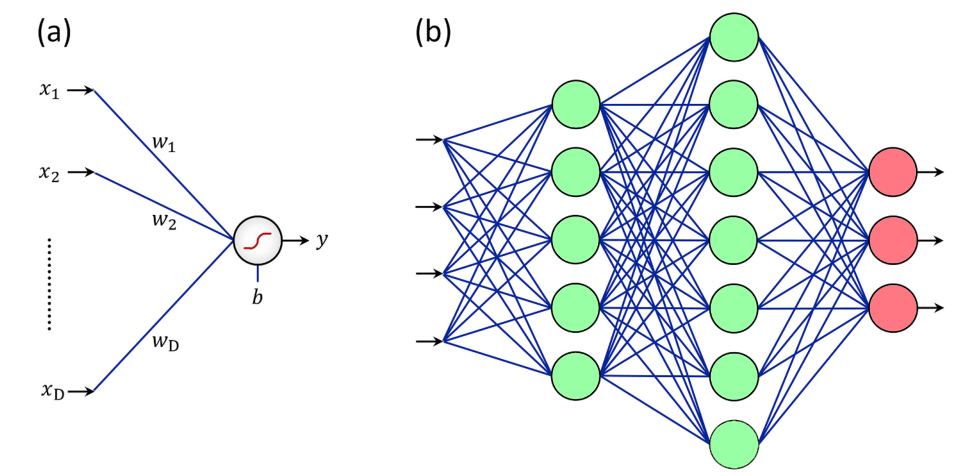
\includegraphics[scale=0.5]{figures/perceptron.png}
            %\hspace*{-3.2cm}
            %\includesvg[inkscapelatex=false,width=1.3\textwidth,keepaspectratio]{figures/overunderfit.svg}
            %% Creator: Matplotlib, PGF backend
%%
%% To include the figure in your LaTeX document, write
%%   \input{<filename>.pgf}
%%
%% Make sure the required packages are loaded in your preamble
%%   \usepackage{pgf}
%%
%% Also ensure that all the required font packages are loaded; for instance,
%% the lmodern package is sometimes necessary when using math font.
%%   \usepackage{lmodern}
%%
%% Figures using additional raster images can only be included by \input if
%% they are in the same directory as the main LaTeX file. For loading figures
%% from other directories you can use the `import` package
%%   \usepackage{import}
%%
%% and then include the figures with
%%   \import{<path to file>}{<filename>.pgf}
%%
%% Matplotlib used the following preamble
%%
\begingroup%
\makeatletter%
\begin{pgfpicture}%
\pgfpathrectangle{\pgfpointorigin}{\pgfqpoint{6.500000in}{2.860000in}}%
\pgfusepath{use as bounding box, clip}%
\begin{pgfscope}%
\pgfsetbuttcap%
\pgfsetmiterjoin%
\definecolor{currentfill}{rgb}{1.000000,1.000000,1.000000}%
\pgfsetfillcolor{currentfill}%
\pgfsetlinewidth{0.000000pt}%
\definecolor{currentstroke}{rgb}{1.000000,1.000000,1.000000}%
\pgfsetstrokecolor{currentstroke}%
\pgfsetdash{}{0pt}%
\pgfpathmoveto{\pgfqpoint{0.000000in}{0.000000in}}%
\pgfpathlineto{\pgfqpoint{6.500000in}{0.000000in}}%
\pgfpathlineto{\pgfqpoint{6.500000in}{2.860000in}}%
\pgfpathlineto{\pgfqpoint{0.000000in}{2.860000in}}%
\pgfpathlineto{\pgfqpoint{0.000000in}{0.000000in}}%
\pgfpathclose%
\pgfusepath{fill}%
\end{pgfscope}%
\begin{pgfscope}%
\pgfsetbuttcap%
\pgfsetmiterjoin%
\definecolor{currentfill}{rgb}{1.000000,1.000000,1.000000}%
\pgfsetfillcolor{currentfill}%
\pgfsetlinewidth{0.000000pt}%
\definecolor{currentstroke}{rgb}{0.000000,0.000000,0.000000}%
\pgfsetstrokecolor{currentstroke}%
\pgfsetstrokeopacity{0.000000}%
\pgfsetdash{}{0pt}%
\pgfpathmoveto{\pgfqpoint{0.812500in}{0.314600in}}%
\pgfpathlineto{\pgfqpoint{2.294118in}{0.314600in}}%
\pgfpathlineto{\pgfqpoint{2.294118in}{2.516800in}}%
\pgfpathlineto{\pgfqpoint{0.812500in}{2.516800in}}%
\pgfpathlineto{\pgfqpoint{0.812500in}{0.314600in}}%
\pgfpathclose%
\pgfusepath{fill}%
\end{pgfscope}%
\begin{pgfscope}%
\pgfpathrectangle{\pgfqpoint{0.812500in}{0.314600in}}{\pgfqpoint{1.481618in}{2.202200in}}%
\pgfusepath{clip}%
\pgfsetbuttcap%
\pgfsetroundjoin%
\definecolor{currentfill}{rgb}{0.121569,0.466667,0.705882}%
\pgfsetfillcolor{currentfill}%
\pgfsetlinewidth{1.003750pt}%
\definecolor{currentstroke}{rgb}{0.000000,0.000000,1.000000}%
\pgfsetstrokecolor{currentstroke}%
\pgfsetdash{}{0pt}%
\pgfsys@defobject{currentmarker}{\pgfqpoint{-0.031056in}{-0.031056in}}{\pgfqpoint{0.031056in}{0.031056in}}{%
\pgfpathmoveto{\pgfqpoint{0.000000in}{-0.031056in}}%
\pgfpathcurveto{\pgfqpoint{0.008236in}{-0.031056in}}{\pgfqpoint{0.016136in}{-0.027784in}}{\pgfqpoint{0.021960in}{-0.021960in}}%
\pgfpathcurveto{\pgfqpoint{0.027784in}{-0.016136in}}{\pgfqpoint{0.031056in}{-0.008236in}}{\pgfqpoint{0.031056in}{0.000000in}}%
\pgfpathcurveto{\pgfqpoint{0.031056in}{0.008236in}}{\pgfqpoint{0.027784in}{0.016136in}}{\pgfqpoint{0.021960in}{0.021960in}}%
\pgfpathcurveto{\pgfqpoint{0.016136in}{0.027784in}}{\pgfqpoint{0.008236in}{0.031056in}}{\pgfqpoint{0.000000in}{0.031056in}}%
\pgfpathcurveto{\pgfqpoint{-0.008236in}{0.031056in}}{\pgfqpoint{-0.016136in}{0.027784in}}{\pgfqpoint{-0.021960in}{0.021960in}}%
\pgfpathcurveto{\pgfqpoint{-0.027784in}{0.016136in}}{\pgfqpoint{-0.031056in}{0.008236in}}{\pgfqpoint{-0.031056in}{0.000000in}}%
\pgfpathcurveto{\pgfqpoint{-0.031056in}{-0.008236in}}{\pgfqpoint{-0.027784in}{-0.016136in}}{\pgfqpoint{-0.021960in}{-0.021960in}}%
\pgfpathcurveto{\pgfqpoint{-0.016136in}{-0.027784in}}{\pgfqpoint{-0.008236in}{-0.031056in}}{\pgfqpoint{0.000000in}{-0.031056in}}%
\pgfpathlineto{\pgfqpoint{0.000000in}{-0.031056in}}%
\pgfpathclose%
\pgfusepath{stroke,fill}%
}%
\begin{pgfscope}%
\pgfsys@transformshift{0.842456in}{1.563258in}%
\pgfsys@useobject{currentmarker}{}%
\end{pgfscope}%
\begin{pgfscope}%
\pgfsys@transformshift{0.917748in}{1.514854in}%
\pgfsys@useobject{currentmarker}{}%
\end{pgfscope}%
\begin{pgfscope}%
\pgfsys@transformshift{0.941592in}{1.885373in}%
\pgfsys@useobject{currentmarker}{}%
\end{pgfscope}%
\begin{pgfscope}%
\pgfsys@transformshift{0.987737in}{1.546770in}%
\pgfsys@useobject{currentmarker}{}%
\end{pgfscope}%
\begin{pgfscope}%
\pgfsys@transformshift{1.024895in}{1.765006in}%
\pgfsys@useobject{currentmarker}{}%
\end{pgfscope}%
\begin{pgfscope}%
\pgfsys@transformshift{1.380614in}{1.930362in}%
\pgfsys@useobject{currentmarker}{}%
\end{pgfscope}%
\begin{pgfscope}%
\pgfsys@transformshift{1.426870in}{2.095084in}%
\pgfsys@useobject{currentmarker}{}%
\end{pgfscope}%
\begin{pgfscope}%
\pgfsys@transformshift{1.440194in}{2.078920in}%
\pgfsys@useobject{currentmarker}{}%
\end{pgfscope}%
\begin{pgfscope}%
\pgfsys@transformshift{1.460837in}{1.918196in}%
\pgfsys@useobject{currentmarker}{}%
\end{pgfscope}%
\begin{pgfscope}%
\pgfsys@transformshift{1.496236in}{1.910520in}%
\pgfsys@useobject{currentmarker}{}%
\end{pgfscope}%
\begin{pgfscope}%
\pgfsys@transformshift{1.585680in}{1.665172in}%
\pgfsys@useobject{currentmarker}{}%
\end{pgfscope}%
\begin{pgfscope}%
\pgfsys@transformshift{1.596120in}{1.530444in}%
\pgfsys@useobject{currentmarker}{}%
\end{pgfscope}%
\begin{pgfscope}%
\pgfsys@transformshift{1.619809in}{1.676287in}%
\pgfsys@useobject{currentmarker}{}%
\end{pgfscope}%
\begin{pgfscope}%
\pgfsys@transformshift{1.625632in}{1.723197in}%
\pgfsys@useobject{currentmarker}{}%
\end{pgfscope}%
\begin{pgfscope}%
\pgfsys@transformshift{1.654125in}{1.797921in}%
\pgfsys@useobject{currentmarker}{}%
\end{pgfscope}%
\begin{pgfscope}%
\pgfsys@transformshift{1.705565in}{1.711391in}%
\pgfsys@useobject{currentmarker}{}%
\end{pgfscope}%
\begin{pgfscope}%
\pgfsys@transformshift{1.760618in}{1.442257in}%
\pgfsys@useobject{currentmarker}{}%
\end{pgfscope}%
\begin{pgfscope}%
\pgfsys@transformshift{1.769468in}{1.436220in}%
\pgfsys@useobject{currentmarker}{}%
\end{pgfscope}%
\begin{pgfscope}%
\pgfsys@transformshift{1.872137in}{1.175450in}%
\pgfsys@useobject{currentmarker}{}%
\end{pgfscope}%
\begin{pgfscope}%
\pgfsys@transformshift{1.965431in}{0.983216in}%
\pgfsys@useobject{currentmarker}{}%
\end{pgfscope}%
\begin{pgfscope}%
\pgfsys@transformshift{1.968946in}{0.946389in}%
\pgfsys@useobject{currentmarker}{}%
\end{pgfscope}%
\begin{pgfscope}%
\pgfsys@transformshift{1.985534in}{1.324505in}%
\pgfsys@useobject{currentmarker}{}%
\end{pgfscope}%
\begin{pgfscope}%
\pgfsys@transformshift{1.996547in}{1.037746in}%
\pgfsys@useobject{currentmarker}{}%
\end{pgfscope}%
\begin{pgfscope}%
\pgfsys@transformshift{2.046124in}{0.979477in}%
\pgfsys@useobject{currentmarker}{}%
\end{pgfscope}%
\begin{pgfscope}%
\pgfsys@transformshift{2.101525in}{0.827304in}%
\pgfsys@useobject{currentmarker}{}%
\end{pgfscope}%
\begin{pgfscope}%
\pgfsys@transformshift{2.133767in}{1.020822in}%
\pgfsys@useobject{currentmarker}{}%
\end{pgfscope}%
\begin{pgfscope}%
\pgfsys@transformshift{2.183880in}{0.720939in}%
\pgfsys@useobject{currentmarker}{}%
\end{pgfscope}%
\begin{pgfscope}%
\pgfsys@transformshift{2.212138in}{0.860334in}%
\pgfsys@useobject{currentmarker}{}%
\end{pgfscope}%
\begin{pgfscope}%
\pgfsys@transformshift{2.240280in}{0.774602in}%
\pgfsys@useobject{currentmarker}{}%
\end{pgfscope}%
\begin{pgfscope}%
\pgfsys@transformshift{2.262438in}{0.910544in}%
\pgfsys@useobject{currentmarker}{}%
\end{pgfscope}%
\end{pgfscope}%
\begin{pgfscope}%
\definecolor{textcolor}{rgb}{0.000000,0.000000,0.000000}%
\pgfsetstrokecolor{textcolor}%
\pgfsetfillcolor{textcolor}%
\pgftext[x=1.553309in,y=0.259044in,,top]{\color{textcolor}\rmfamily\fontsize{10.000000}{12.000000}\selectfont x}%
\end{pgfscope}%
\begin{pgfscope}%
\definecolor{textcolor}{rgb}{0.000000,0.000000,0.000000}%
\pgfsetstrokecolor{textcolor}%
\pgfsetfillcolor{textcolor}%
\pgftext[x=0.756944in,y=1.415700in,,bottom,rotate=90.000000]{\color{textcolor}\rmfamily\fontsize{10.000000}{12.000000}\selectfont y}%
\end{pgfscope}%
\begin{pgfscope}%
\pgfpathrectangle{\pgfqpoint{0.812500in}{0.314600in}}{\pgfqpoint{1.481618in}{2.202200in}}%
\pgfusepath{clip}%
\pgfsetrectcap%
\pgfsetroundjoin%
\pgfsetlinewidth{1.505625pt}%
\definecolor{currentstroke}{rgb}{0.121569,0.466667,0.705882}%
\pgfsetstrokecolor{currentstroke}%
\pgfsetdash{}{0pt}%
\pgfpathmoveto{\pgfqpoint{0.812500in}{2.083377in}}%
\pgfpathlineto{\pgfqpoint{0.827466in}{2.071935in}}%
\pgfpathlineto{\pgfqpoint{0.842432in}{2.060492in}}%
\pgfpathlineto{\pgfqpoint{0.857398in}{2.049050in}}%
\pgfpathlineto{\pgfqpoint{0.872363in}{2.037607in}}%
\pgfpathlineto{\pgfqpoint{0.887329in}{2.026165in}}%
\pgfpathlineto{\pgfqpoint{0.902295in}{2.014723in}}%
\pgfpathlineto{\pgfqpoint{0.917261in}{2.003280in}}%
\pgfpathlineto{\pgfqpoint{0.932227in}{1.991838in}}%
\pgfpathlineto{\pgfqpoint{0.947193in}{1.980395in}}%
\pgfpathlineto{\pgfqpoint{0.962158in}{1.968953in}}%
\pgfpathlineto{\pgfqpoint{0.977124in}{1.957511in}}%
\pgfpathlineto{\pgfqpoint{0.992090in}{1.946068in}}%
\pgfpathlineto{\pgfqpoint{1.007056in}{1.934626in}}%
\pgfpathlineto{\pgfqpoint{1.022022in}{1.923183in}}%
\pgfpathlineto{\pgfqpoint{1.036988in}{1.911741in}}%
\pgfpathlineto{\pgfqpoint{1.051953in}{1.900299in}}%
\pgfpathlineto{\pgfqpoint{1.066919in}{1.888856in}}%
\pgfpathlineto{\pgfqpoint{1.081885in}{1.877414in}}%
\pgfpathlineto{\pgfqpoint{1.096851in}{1.865971in}}%
\pgfpathlineto{\pgfqpoint{1.111817in}{1.854529in}}%
\pgfpathlineto{\pgfqpoint{1.126783in}{1.843087in}}%
\pgfpathlineto{\pgfqpoint{1.141748in}{1.831644in}}%
\pgfpathlineto{\pgfqpoint{1.156714in}{1.820202in}}%
\pgfpathlineto{\pgfqpoint{1.171680in}{1.808759in}}%
\pgfpathlineto{\pgfqpoint{1.186646in}{1.797317in}}%
\pgfpathlineto{\pgfqpoint{1.201612in}{1.785875in}}%
\pgfpathlineto{\pgfqpoint{1.216578in}{1.774432in}}%
\pgfpathlineto{\pgfqpoint{1.231543in}{1.762990in}}%
\pgfpathlineto{\pgfqpoint{1.246509in}{1.751547in}}%
\pgfpathlineto{\pgfqpoint{1.261475in}{1.740105in}}%
\pgfpathlineto{\pgfqpoint{1.276441in}{1.728663in}}%
\pgfpathlineto{\pgfqpoint{1.291407in}{1.717220in}}%
\pgfpathlineto{\pgfqpoint{1.306373in}{1.705778in}}%
\pgfpathlineto{\pgfqpoint{1.321338in}{1.694335in}}%
\pgfpathlineto{\pgfqpoint{1.336304in}{1.682893in}}%
\pgfpathlineto{\pgfqpoint{1.351270in}{1.671451in}}%
\pgfpathlineto{\pgfqpoint{1.366236in}{1.660008in}}%
\pgfpathlineto{\pgfqpoint{1.381202in}{1.648566in}}%
\pgfpathlineto{\pgfqpoint{1.396168in}{1.637123in}}%
\pgfpathlineto{\pgfqpoint{1.411133in}{1.625681in}}%
\pgfpathlineto{\pgfqpoint{1.426099in}{1.614239in}}%
\pgfpathlineto{\pgfqpoint{1.441065in}{1.602796in}}%
\pgfpathlineto{\pgfqpoint{1.456031in}{1.591354in}}%
\pgfpathlineto{\pgfqpoint{1.470997in}{1.579911in}}%
\pgfpathlineto{\pgfqpoint{1.485963in}{1.568469in}}%
\pgfpathlineto{\pgfqpoint{1.500928in}{1.557027in}}%
\pgfpathlineto{\pgfqpoint{1.515894in}{1.545584in}}%
\pgfpathlineto{\pgfqpoint{1.530860in}{1.534142in}}%
\pgfpathlineto{\pgfqpoint{1.545826in}{1.522699in}}%
\pgfpathlineto{\pgfqpoint{1.560792in}{1.511257in}}%
\pgfpathlineto{\pgfqpoint{1.575758in}{1.499815in}}%
\pgfpathlineto{\pgfqpoint{1.590723in}{1.488372in}}%
\pgfpathlineto{\pgfqpoint{1.605689in}{1.476930in}}%
\pgfpathlineto{\pgfqpoint{1.620655in}{1.465487in}}%
\pgfpathlineto{\pgfqpoint{1.635621in}{1.454045in}}%
\pgfpathlineto{\pgfqpoint{1.650587in}{1.442603in}}%
\pgfpathlineto{\pgfqpoint{1.665553in}{1.431160in}}%
\pgfpathlineto{\pgfqpoint{1.680518in}{1.419718in}}%
\pgfpathlineto{\pgfqpoint{1.695484in}{1.408275in}}%
\pgfpathlineto{\pgfqpoint{1.710450in}{1.396833in}}%
\pgfpathlineto{\pgfqpoint{1.725416in}{1.385391in}}%
\pgfpathlineto{\pgfqpoint{1.740382in}{1.373948in}}%
\pgfpathlineto{\pgfqpoint{1.755348in}{1.362506in}}%
\pgfpathlineto{\pgfqpoint{1.770313in}{1.351064in}}%
\pgfpathlineto{\pgfqpoint{1.785279in}{1.339621in}}%
\pgfpathlineto{\pgfqpoint{1.800245in}{1.328179in}}%
\pgfpathlineto{\pgfqpoint{1.815211in}{1.316736in}}%
\pgfpathlineto{\pgfqpoint{1.830177in}{1.305294in}}%
\pgfpathlineto{\pgfqpoint{1.845143in}{1.293852in}}%
\pgfpathlineto{\pgfqpoint{1.860108in}{1.282409in}}%
\pgfpathlineto{\pgfqpoint{1.875074in}{1.270967in}}%
\pgfpathlineto{\pgfqpoint{1.890040in}{1.259524in}}%
\pgfpathlineto{\pgfqpoint{1.905006in}{1.248082in}}%
\pgfpathlineto{\pgfqpoint{1.919972in}{1.236640in}}%
\pgfpathlineto{\pgfqpoint{1.934938in}{1.225197in}}%
\pgfpathlineto{\pgfqpoint{1.949903in}{1.213755in}}%
\pgfpathlineto{\pgfqpoint{1.964869in}{1.202312in}}%
\pgfpathlineto{\pgfqpoint{1.979835in}{1.190870in}}%
\pgfpathlineto{\pgfqpoint{1.994801in}{1.179428in}}%
\pgfpathlineto{\pgfqpoint{2.009767in}{1.167985in}}%
\pgfpathlineto{\pgfqpoint{2.024733in}{1.156543in}}%
\pgfpathlineto{\pgfqpoint{2.039698in}{1.145100in}}%
\pgfpathlineto{\pgfqpoint{2.054664in}{1.133658in}}%
\pgfpathlineto{\pgfqpoint{2.069630in}{1.122216in}}%
\pgfpathlineto{\pgfqpoint{2.084596in}{1.110773in}}%
\pgfpathlineto{\pgfqpoint{2.099562in}{1.099331in}}%
\pgfpathlineto{\pgfqpoint{2.114528in}{1.087888in}}%
\pgfpathlineto{\pgfqpoint{2.129493in}{1.076446in}}%
\pgfpathlineto{\pgfqpoint{2.144459in}{1.065004in}}%
\pgfpathlineto{\pgfqpoint{2.159425in}{1.053561in}}%
\pgfpathlineto{\pgfqpoint{2.174391in}{1.042119in}}%
\pgfpathlineto{\pgfqpoint{2.189357in}{1.030676in}}%
\pgfpathlineto{\pgfqpoint{2.204323in}{1.019234in}}%
\pgfpathlineto{\pgfqpoint{2.219288in}{1.007792in}}%
\pgfpathlineto{\pgfqpoint{2.234254in}{0.996349in}}%
\pgfpathlineto{\pgfqpoint{2.249220in}{0.984907in}}%
\pgfpathlineto{\pgfqpoint{2.264186in}{0.973464in}}%
\pgfpathlineto{\pgfqpoint{2.279152in}{0.962022in}}%
\pgfpathlineto{\pgfqpoint{2.294118in}{0.950580in}}%
\pgfusepath{stroke}%
\end{pgfscope}%
\begin{pgfscope}%
\pgfpathrectangle{\pgfqpoint{0.812500in}{0.314600in}}{\pgfqpoint{1.481618in}{2.202200in}}%
\pgfusepath{clip}%
\pgfsetrectcap%
\pgfsetroundjoin%
\pgfsetlinewidth{1.505625pt}%
\definecolor{currentstroke}{rgb}{1.000000,0.498039,0.054902}%
\pgfsetstrokecolor{currentstroke}%
\pgfsetdash{}{0pt}%
\pgfpathmoveto{\pgfqpoint{0.812500in}{1.415700in}}%
\pgfpathlineto{\pgfqpoint{0.827466in}{1.441896in}}%
\pgfpathlineto{\pgfqpoint{0.842432in}{1.468033in}}%
\pgfpathlineto{\pgfqpoint{0.857398in}{1.494051in}}%
\pgfpathlineto{\pgfqpoint{0.872363in}{1.519892in}}%
\pgfpathlineto{\pgfqpoint{0.887329in}{1.545497in}}%
\pgfpathlineto{\pgfqpoint{0.902295in}{1.570808in}}%
\pgfpathlineto{\pgfqpoint{0.917261in}{1.595767in}}%
\pgfpathlineto{\pgfqpoint{0.932227in}{1.620319in}}%
\pgfpathlineto{\pgfqpoint{0.947193in}{1.644407in}}%
\pgfpathlineto{\pgfqpoint{0.962158in}{1.667977in}}%
\pgfpathlineto{\pgfqpoint{0.977124in}{1.690975in}}%
\pgfpathlineto{\pgfqpoint{0.992090in}{1.713350in}}%
\pgfpathlineto{\pgfqpoint{1.007056in}{1.735050in}}%
\pgfpathlineto{\pgfqpoint{1.022022in}{1.756027in}}%
\pgfpathlineto{\pgfqpoint{1.036988in}{1.776234in}}%
\pgfpathlineto{\pgfqpoint{1.051953in}{1.795623in}}%
\pgfpathlineto{\pgfqpoint{1.066919in}{1.814152in}}%
\pgfpathlineto{\pgfqpoint{1.081885in}{1.831778in}}%
\pgfpathlineto{\pgfqpoint{1.096851in}{1.848462in}}%
\pgfpathlineto{\pgfqpoint{1.111817in}{1.864165in}}%
\pgfpathlineto{\pgfqpoint{1.126783in}{1.878852in}}%
\pgfpathlineto{\pgfqpoint{1.141748in}{1.892490in}}%
\pgfpathlineto{\pgfqpoint{1.156714in}{1.905048in}}%
\pgfpathlineto{\pgfqpoint{1.171680in}{1.916498in}}%
\pgfpathlineto{\pgfqpoint{1.186646in}{1.926813in}}%
\pgfpathlineto{\pgfqpoint{1.201612in}{1.935970in}}%
\pgfpathlineto{\pgfqpoint{1.216578in}{1.943949in}}%
\pgfpathlineto{\pgfqpoint{1.231543in}{1.950731in}}%
\pgfpathlineto{\pgfqpoint{1.246509in}{1.956301in}}%
\pgfpathlineto{\pgfqpoint{1.261475in}{1.960646in}}%
\pgfpathlineto{\pgfqpoint{1.276441in}{1.963757in}}%
\pgfpathlineto{\pgfqpoint{1.291407in}{1.965626in}}%
\pgfpathlineto{\pgfqpoint{1.306373in}{1.966250in}}%
\pgfpathlineto{\pgfqpoint{1.321338in}{1.965626in}}%
\pgfpathlineto{\pgfqpoint{1.336304in}{1.963757in}}%
\pgfpathlineto{\pgfqpoint{1.351270in}{1.960646in}}%
\pgfpathlineto{\pgfqpoint{1.366236in}{1.956301in}}%
\pgfpathlineto{\pgfqpoint{1.381202in}{1.950731in}}%
\pgfpathlineto{\pgfqpoint{1.396168in}{1.943949in}}%
\pgfpathlineto{\pgfqpoint{1.411133in}{1.935970in}}%
\pgfpathlineto{\pgfqpoint{1.426099in}{1.926813in}}%
\pgfpathlineto{\pgfqpoint{1.441065in}{1.916498in}}%
\pgfpathlineto{\pgfqpoint{1.456031in}{1.905048in}}%
\pgfpathlineto{\pgfqpoint{1.470997in}{1.892490in}}%
\pgfpathlineto{\pgfqpoint{1.485963in}{1.878852in}}%
\pgfpathlineto{\pgfqpoint{1.500928in}{1.864165in}}%
\pgfpathlineto{\pgfqpoint{1.515894in}{1.848462in}}%
\pgfpathlineto{\pgfqpoint{1.530860in}{1.831778in}}%
\pgfpathlineto{\pgfqpoint{1.545826in}{1.814152in}}%
\pgfpathlineto{\pgfqpoint{1.560792in}{1.795623in}}%
\pgfpathlineto{\pgfqpoint{1.575758in}{1.776234in}}%
\pgfpathlineto{\pgfqpoint{1.590723in}{1.756027in}}%
\pgfpathlineto{\pgfqpoint{1.605689in}{1.735050in}}%
\pgfpathlineto{\pgfqpoint{1.620655in}{1.713350in}}%
\pgfpathlineto{\pgfqpoint{1.635621in}{1.690975in}}%
\pgfpathlineto{\pgfqpoint{1.650587in}{1.667977in}}%
\pgfpathlineto{\pgfqpoint{1.665553in}{1.644407in}}%
\pgfpathlineto{\pgfqpoint{1.680518in}{1.620319in}}%
\pgfpathlineto{\pgfqpoint{1.695484in}{1.595767in}}%
\pgfpathlineto{\pgfqpoint{1.710450in}{1.570808in}}%
\pgfpathlineto{\pgfqpoint{1.725416in}{1.545497in}}%
\pgfpathlineto{\pgfqpoint{1.740382in}{1.519892in}}%
\pgfpathlineto{\pgfqpoint{1.755348in}{1.494051in}}%
\pgfpathlineto{\pgfqpoint{1.770313in}{1.468033in}}%
\pgfpathlineto{\pgfqpoint{1.785279in}{1.441896in}}%
\pgfpathlineto{\pgfqpoint{1.800245in}{1.415700in}}%
\pgfpathlineto{\pgfqpoint{1.815211in}{1.389504in}}%
\pgfpathlineto{\pgfqpoint{1.830177in}{1.363367in}}%
\pgfpathlineto{\pgfqpoint{1.845143in}{1.337349in}}%
\pgfpathlineto{\pgfqpoint{1.860108in}{1.311508in}}%
\pgfpathlineto{\pgfqpoint{1.875074in}{1.285903in}}%
\pgfpathlineto{\pgfqpoint{1.890040in}{1.260592in}}%
\pgfpathlineto{\pgfqpoint{1.905006in}{1.235633in}}%
\pgfpathlineto{\pgfqpoint{1.919972in}{1.211081in}}%
\pgfpathlineto{\pgfqpoint{1.934938in}{1.186993in}}%
\pgfpathlineto{\pgfqpoint{1.949903in}{1.163423in}}%
\pgfpathlineto{\pgfqpoint{1.964869in}{1.140425in}}%
\pgfpathlineto{\pgfqpoint{1.979835in}{1.118050in}}%
\pgfpathlineto{\pgfqpoint{1.994801in}{1.096350in}}%
\pgfpathlineto{\pgfqpoint{2.009767in}{1.075373in}}%
\pgfpathlineto{\pgfqpoint{2.024733in}{1.055166in}}%
\pgfpathlineto{\pgfqpoint{2.039698in}{1.035777in}}%
\pgfpathlineto{\pgfqpoint{2.054664in}{1.017248in}}%
\pgfpathlineto{\pgfqpoint{2.069630in}{0.999622in}}%
\pgfpathlineto{\pgfqpoint{2.084596in}{0.982938in}}%
\pgfpathlineto{\pgfqpoint{2.099562in}{0.967235in}}%
\pgfpathlineto{\pgfqpoint{2.114528in}{0.952548in}}%
\pgfpathlineto{\pgfqpoint{2.129493in}{0.938910in}}%
\pgfpathlineto{\pgfqpoint{2.144459in}{0.926352in}}%
\pgfpathlineto{\pgfqpoint{2.159425in}{0.914902in}}%
\pgfpathlineto{\pgfqpoint{2.174391in}{0.904587in}}%
\pgfpathlineto{\pgfqpoint{2.189357in}{0.895430in}}%
\pgfpathlineto{\pgfqpoint{2.204323in}{0.887451in}}%
\pgfpathlineto{\pgfqpoint{2.219288in}{0.880669in}}%
\pgfpathlineto{\pgfqpoint{2.234254in}{0.875099in}}%
\pgfpathlineto{\pgfqpoint{2.249220in}{0.870754in}}%
\pgfpathlineto{\pgfqpoint{2.264186in}{0.867643in}}%
\pgfpathlineto{\pgfqpoint{2.279152in}{0.865774in}}%
\pgfpathlineto{\pgfqpoint{2.294118in}{0.865150in}}%
\pgfusepath{stroke}%
\end{pgfscope}%
\begin{pgfscope}%
\pgfsetrectcap%
\pgfsetmiterjoin%
\pgfsetlinewidth{0.803000pt}%
\definecolor{currentstroke}{rgb}{0.000000,0.000000,0.000000}%
\pgfsetstrokecolor{currentstroke}%
\pgfsetdash{}{0pt}%
\pgfpathmoveto{\pgfqpoint{0.812500in}{0.314600in}}%
\pgfpathlineto{\pgfqpoint{0.812500in}{2.516800in}}%
\pgfusepath{stroke}%
\end{pgfscope}%
\begin{pgfscope}%
\pgfsetrectcap%
\pgfsetmiterjoin%
\pgfsetlinewidth{0.803000pt}%
\definecolor{currentstroke}{rgb}{0.000000,0.000000,0.000000}%
\pgfsetstrokecolor{currentstroke}%
\pgfsetdash{}{0pt}%
\pgfpathmoveto{\pgfqpoint{2.294118in}{0.314600in}}%
\pgfpathlineto{\pgfqpoint{2.294118in}{2.516800in}}%
\pgfusepath{stroke}%
\end{pgfscope}%
\begin{pgfscope}%
\pgfsetrectcap%
\pgfsetmiterjoin%
\pgfsetlinewidth{0.803000pt}%
\definecolor{currentstroke}{rgb}{0.000000,0.000000,0.000000}%
\pgfsetstrokecolor{currentstroke}%
\pgfsetdash{}{0pt}%
\pgfpathmoveto{\pgfqpoint{0.812500in}{0.314600in}}%
\pgfpathlineto{\pgfqpoint{2.294118in}{0.314600in}}%
\pgfusepath{stroke}%
\end{pgfscope}%
\begin{pgfscope}%
\pgfsetrectcap%
\pgfsetmiterjoin%
\pgfsetlinewidth{0.803000pt}%
\definecolor{currentstroke}{rgb}{0.000000,0.000000,0.000000}%
\pgfsetstrokecolor{currentstroke}%
\pgfsetdash{}{0pt}%
\pgfpathmoveto{\pgfqpoint{0.812500in}{2.516800in}}%
\pgfpathlineto{\pgfqpoint{2.294118in}{2.516800in}}%
\pgfusepath{stroke}%
\end{pgfscope}%
\begin{pgfscope}%
\definecolor{textcolor}{rgb}{0.000000,0.000000,0.000000}%
\pgfsetstrokecolor{textcolor}%
\pgfsetfillcolor{textcolor}%
\pgftext[x=1.553309in,y=2.600133in,,base]{\color{textcolor}\rmfamily\fontsize{16.000000}{19.200000}\selectfont Underfit}%
\end{pgfscope}%
\begin{pgfscope}%
\pgfsetbuttcap%
\pgfsetmiterjoin%
\definecolor{currentfill}{rgb}{1.000000,1.000000,1.000000}%
\pgfsetfillcolor{currentfill}%
\pgfsetlinewidth{0.000000pt}%
\definecolor{currentstroke}{rgb}{0.000000,0.000000,0.000000}%
\pgfsetstrokecolor{currentstroke}%
\pgfsetstrokeopacity{0.000000}%
\pgfsetdash{}{0pt}%
\pgfpathmoveto{\pgfqpoint{2.590441in}{0.314600in}}%
\pgfpathlineto{\pgfqpoint{4.072059in}{0.314600in}}%
\pgfpathlineto{\pgfqpoint{4.072059in}{2.516800in}}%
\pgfpathlineto{\pgfqpoint{2.590441in}{2.516800in}}%
\pgfpathlineto{\pgfqpoint{2.590441in}{0.314600in}}%
\pgfpathclose%
\pgfusepath{fill}%
\end{pgfscope}%
\begin{pgfscope}%
\pgfpathrectangle{\pgfqpoint{2.590441in}{0.314600in}}{\pgfqpoint{1.481618in}{2.202200in}}%
\pgfusepath{clip}%
\pgfsetbuttcap%
\pgfsetroundjoin%
\definecolor{currentfill}{rgb}{0.121569,0.466667,0.705882}%
\pgfsetfillcolor{currentfill}%
\pgfsetlinewidth{1.003750pt}%
\definecolor{currentstroke}{rgb}{0.000000,0.000000,1.000000}%
\pgfsetstrokecolor{currentstroke}%
\pgfsetdash{}{0pt}%
\pgfsys@defobject{currentmarker}{\pgfqpoint{-0.031056in}{-0.031056in}}{\pgfqpoint{0.031056in}{0.031056in}}{%
\pgfpathmoveto{\pgfqpoint{0.000000in}{-0.031056in}}%
\pgfpathcurveto{\pgfqpoint{0.008236in}{-0.031056in}}{\pgfqpoint{0.016136in}{-0.027784in}}{\pgfqpoint{0.021960in}{-0.021960in}}%
\pgfpathcurveto{\pgfqpoint{0.027784in}{-0.016136in}}{\pgfqpoint{0.031056in}{-0.008236in}}{\pgfqpoint{0.031056in}{0.000000in}}%
\pgfpathcurveto{\pgfqpoint{0.031056in}{0.008236in}}{\pgfqpoint{0.027784in}{0.016136in}}{\pgfqpoint{0.021960in}{0.021960in}}%
\pgfpathcurveto{\pgfqpoint{0.016136in}{0.027784in}}{\pgfqpoint{0.008236in}{0.031056in}}{\pgfqpoint{0.000000in}{0.031056in}}%
\pgfpathcurveto{\pgfqpoint{-0.008236in}{0.031056in}}{\pgfqpoint{-0.016136in}{0.027784in}}{\pgfqpoint{-0.021960in}{0.021960in}}%
\pgfpathcurveto{\pgfqpoint{-0.027784in}{0.016136in}}{\pgfqpoint{-0.031056in}{0.008236in}}{\pgfqpoint{-0.031056in}{0.000000in}}%
\pgfpathcurveto{\pgfqpoint{-0.031056in}{-0.008236in}}{\pgfqpoint{-0.027784in}{-0.016136in}}{\pgfqpoint{-0.021960in}{-0.021960in}}%
\pgfpathcurveto{\pgfqpoint{-0.016136in}{-0.027784in}}{\pgfqpoint{-0.008236in}{-0.031056in}}{\pgfqpoint{0.000000in}{-0.031056in}}%
\pgfpathlineto{\pgfqpoint{0.000000in}{-0.031056in}}%
\pgfpathclose%
\pgfusepath{stroke,fill}%
}%
\begin{pgfscope}%
\pgfsys@transformshift{2.620397in}{1.563258in}%
\pgfsys@useobject{currentmarker}{}%
\end{pgfscope}%
\begin{pgfscope}%
\pgfsys@transformshift{2.695689in}{1.514854in}%
\pgfsys@useobject{currentmarker}{}%
\end{pgfscope}%
\begin{pgfscope}%
\pgfsys@transformshift{2.719533in}{1.885373in}%
\pgfsys@useobject{currentmarker}{}%
\end{pgfscope}%
\begin{pgfscope}%
\pgfsys@transformshift{2.765679in}{1.546770in}%
\pgfsys@useobject{currentmarker}{}%
\end{pgfscope}%
\begin{pgfscope}%
\pgfsys@transformshift{2.802836in}{1.765006in}%
\pgfsys@useobject{currentmarker}{}%
\end{pgfscope}%
\begin{pgfscope}%
\pgfsys@transformshift{3.158555in}{1.930362in}%
\pgfsys@useobject{currentmarker}{}%
\end{pgfscope}%
\begin{pgfscope}%
\pgfsys@transformshift{3.204812in}{2.095084in}%
\pgfsys@useobject{currentmarker}{}%
\end{pgfscope}%
\begin{pgfscope}%
\pgfsys@transformshift{3.218136in}{2.078920in}%
\pgfsys@useobject{currentmarker}{}%
\end{pgfscope}%
\begin{pgfscope}%
\pgfsys@transformshift{3.238778in}{1.918196in}%
\pgfsys@useobject{currentmarker}{}%
\end{pgfscope}%
\begin{pgfscope}%
\pgfsys@transformshift{3.274177in}{1.910520in}%
\pgfsys@useobject{currentmarker}{}%
\end{pgfscope}%
\begin{pgfscope}%
\pgfsys@transformshift{3.363621in}{1.665172in}%
\pgfsys@useobject{currentmarker}{}%
\end{pgfscope}%
\begin{pgfscope}%
\pgfsys@transformshift{3.374061in}{1.530444in}%
\pgfsys@useobject{currentmarker}{}%
\end{pgfscope}%
\begin{pgfscope}%
\pgfsys@transformshift{3.397750in}{1.676287in}%
\pgfsys@useobject{currentmarker}{}%
\end{pgfscope}%
\begin{pgfscope}%
\pgfsys@transformshift{3.403573in}{1.723197in}%
\pgfsys@useobject{currentmarker}{}%
\end{pgfscope}%
\begin{pgfscope}%
\pgfsys@transformshift{3.432066in}{1.797921in}%
\pgfsys@useobject{currentmarker}{}%
\end{pgfscope}%
\begin{pgfscope}%
\pgfsys@transformshift{3.483506in}{1.711391in}%
\pgfsys@useobject{currentmarker}{}%
\end{pgfscope}%
\begin{pgfscope}%
\pgfsys@transformshift{3.538559in}{1.442257in}%
\pgfsys@useobject{currentmarker}{}%
\end{pgfscope}%
\begin{pgfscope}%
\pgfsys@transformshift{3.547409in}{1.436220in}%
\pgfsys@useobject{currentmarker}{}%
\end{pgfscope}%
\begin{pgfscope}%
\pgfsys@transformshift{3.650078in}{1.175450in}%
\pgfsys@useobject{currentmarker}{}%
\end{pgfscope}%
\begin{pgfscope}%
\pgfsys@transformshift{3.743372in}{0.983216in}%
\pgfsys@useobject{currentmarker}{}%
\end{pgfscope}%
\begin{pgfscope}%
\pgfsys@transformshift{3.746887in}{0.946389in}%
\pgfsys@useobject{currentmarker}{}%
\end{pgfscope}%
\begin{pgfscope}%
\pgfsys@transformshift{3.763475in}{1.324505in}%
\pgfsys@useobject{currentmarker}{}%
\end{pgfscope}%
\begin{pgfscope}%
\pgfsys@transformshift{3.774489in}{1.037746in}%
\pgfsys@useobject{currentmarker}{}%
\end{pgfscope}%
\begin{pgfscope}%
\pgfsys@transformshift{3.824065in}{0.979477in}%
\pgfsys@useobject{currentmarker}{}%
\end{pgfscope}%
\begin{pgfscope}%
\pgfsys@transformshift{3.879467in}{0.827304in}%
\pgfsys@useobject{currentmarker}{}%
\end{pgfscope}%
\begin{pgfscope}%
\pgfsys@transformshift{3.911708in}{1.020822in}%
\pgfsys@useobject{currentmarker}{}%
\end{pgfscope}%
\begin{pgfscope}%
\pgfsys@transformshift{3.961821in}{0.720939in}%
\pgfsys@useobject{currentmarker}{}%
\end{pgfscope}%
\begin{pgfscope}%
\pgfsys@transformshift{3.990079in}{0.860334in}%
\pgfsys@useobject{currentmarker}{}%
\end{pgfscope}%
\begin{pgfscope}%
\pgfsys@transformshift{4.018221in}{0.774602in}%
\pgfsys@useobject{currentmarker}{}%
\end{pgfscope}%
\begin{pgfscope}%
\pgfsys@transformshift{4.040379in}{0.910544in}%
\pgfsys@useobject{currentmarker}{}%
\end{pgfscope}%
\end{pgfscope}%
\begin{pgfscope}%
\definecolor{textcolor}{rgb}{0.000000,0.000000,0.000000}%
\pgfsetstrokecolor{textcolor}%
\pgfsetfillcolor{textcolor}%
\pgftext[x=3.331250in,y=0.259044in,,top]{\color{textcolor}\rmfamily\fontsize{10.000000}{12.000000}\selectfont x}%
\end{pgfscope}%
\begin{pgfscope}%
\definecolor{textcolor}{rgb}{0.000000,0.000000,0.000000}%
\pgfsetstrokecolor{textcolor}%
\pgfsetfillcolor{textcolor}%
\pgftext[x=2.534886in,y=1.415700in,,bottom,rotate=90.000000]{\color{textcolor}\rmfamily\fontsize{10.000000}{12.000000}\selectfont y}%
\end{pgfscope}%
\begin{pgfscope}%
\pgfpathrectangle{\pgfqpoint{2.590441in}{0.314600in}}{\pgfqpoint{1.481618in}{2.202200in}}%
\pgfusepath{clip}%
\pgfsetrectcap%
\pgfsetroundjoin%
\pgfsetlinewidth{1.505625pt}%
\definecolor{currentstroke}{rgb}{0.121569,0.466667,0.705882}%
\pgfsetstrokecolor{currentstroke}%
\pgfsetdash{}{0pt}%
\pgfpathmoveto{\pgfqpoint{2.590441in}{1.486783in}}%
\pgfpathlineto{\pgfqpoint{2.605407in}{1.506369in}}%
\pgfpathlineto{\pgfqpoint{2.620373in}{1.526427in}}%
\pgfpathlineto{\pgfqpoint{2.635339in}{1.546865in}}%
\pgfpathlineto{\pgfqpoint{2.650305in}{1.567592in}}%
\pgfpathlineto{\pgfqpoint{2.665270in}{1.588518in}}%
\pgfpathlineto{\pgfqpoint{2.680236in}{1.609560in}}%
\pgfpathlineto{\pgfqpoint{2.695202in}{1.630632in}}%
\pgfpathlineto{\pgfqpoint{2.710168in}{1.651657in}}%
\pgfpathlineto{\pgfqpoint{2.725134in}{1.672554in}}%
\pgfpathlineto{\pgfqpoint{2.740100in}{1.693250in}}%
\pgfpathlineto{\pgfqpoint{2.755065in}{1.713671in}}%
\pgfpathlineto{\pgfqpoint{2.770031in}{1.733748in}}%
\pgfpathlineto{\pgfqpoint{2.784997in}{1.753414in}}%
\pgfpathlineto{\pgfqpoint{2.799963in}{1.772603in}}%
\pgfpathlineto{\pgfqpoint{2.814929in}{1.791254in}}%
\pgfpathlineto{\pgfqpoint{2.829895in}{1.809307in}}%
\pgfpathlineto{\pgfqpoint{2.844860in}{1.826705in}}%
\pgfpathlineto{\pgfqpoint{2.859826in}{1.843395in}}%
\pgfpathlineto{\pgfqpoint{2.874792in}{1.859323in}}%
\pgfpathlineto{\pgfqpoint{2.889758in}{1.874443in}}%
\pgfpathlineto{\pgfqpoint{2.904724in}{1.888706in}}%
\pgfpathlineto{\pgfqpoint{2.919690in}{1.902069in}}%
\pgfpathlineto{\pgfqpoint{2.934655in}{1.914491in}}%
\pgfpathlineto{\pgfqpoint{2.949621in}{1.925934in}}%
\pgfpathlineto{\pgfqpoint{2.964587in}{1.936361in}}%
\pgfpathlineto{\pgfqpoint{2.979553in}{1.945740in}}%
\pgfpathlineto{\pgfqpoint{2.994519in}{1.954039in}}%
\pgfpathlineto{\pgfqpoint{3.009485in}{1.961230in}}%
\pgfpathlineto{\pgfqpoint{3.024450in}{1.967288in}}%
\pgfpathlineto{\pgfqpoint{3.039416in}{1.972191in}}%
\pgfpathlineto{\pgfqpoint{3.054382in}{1.975917in}}%
\pgfpathlineto{\pgfqpoint{3.069348in}{1.978449in}}%
\pgfpathlineto{\pgfqpoint{3.084314in}{1.979773in}}%
\pgfpathlineto{\pgfqpoint{3.099280in}{1.979875in}}%
\pgfpathlineto{\pgfqpoint{3.114245in}{1.978746in}}%
\pgfpathlineto{\pgfqpoint{3.129211in}{1.976379in}}%
\pgfpathlineto{\pgfqpoint{3.144177in}{1.972770in}}%
\pgfpathlineto{\pgfqpoint{3.159143in}{1.967916in}}%
\pgfpathlineto{\pgfqpoint{3.174109in}{1.961817in}}%
\pgfpathlineto{\pgfqpoint{3.189075in}{1.954478in}}%
\pgfpathlineto{\pgfqpoint{3.204040in}{1.945905in}}%
\pgfpathlineto{\pgfqpoint{3.219006in}{1.936104in}}%
\pgfpathlineto{\pgfqpoint{3.233972in}{1.925089in}}%
\pgfpathlineto{\pgfqpoint{3.248938in}{1.912873in}}%
\pgfpathlineto{\pgfqpoint{3.263904in}{1.899471in}}%
\pgfpathlineto{\pgfqpoint{3.278870in}{1.884904in}}%
\pgfpathlineto{\pgfqpoint{3.293835in}{1.869192in}}%
\pgfpathlineto{\pgfqpoint{3.308801in}{1.852359in}}%
\pgfpathlineto{\pgfqpoint{3.323767in}{1.834434in}}%
\pgfpathlineto{\pgfqpoint{3.338733in}{1.815444in}}%
\pgfpathlineto{\pgfqpoint{3.353699in}{1.795423in}}%
\pgfpathlineto{\pgfqpoint{3.368665in}{1.774405in}}%
\pgfpathlineto{\pgfqpoint{3.383630in}{1.752426in}}%
\pgfpathlineto{\pgfqpoint{3.398596in}{1.729528in}}%
\pgfpathlineto{\pgfqpoint{3.413562in}{1.705752in}}%
\pgfpathlineto{\pgfqpoint{3.428528in}{1.681144in}}%
\pgfpathlineto{\pgfqpoint{3.443494in}{1.655751in}}%
\pgfpathlineto{\pgfqpoint{3.458460in}{1.629625in}}%
\pgfpathlineto{\pgfqpoint{3.473425in}{1.602817in}}%
\pgfpathlineto{\pgfqpoint{3.488391in}{1.575383in}}%
\pgfpathlineto{\pgfqpoint{3.503357in}{1.547382in}}%
\pgfpathlineto{\pgfqpoint{3.518323in}{1.518875in}}%
\pgfpathlineto{\pgfqpoint{3.533289in}{1.489924in}}%
\pgfpathlineto{\pgfqpoint{3.548255in}{1.460596in}}%
\pgfpathlineto{\pgfqpoint{3.563220in}{1.430961in}}%
\pgfpathlineto{\pgfqpoint{3.578186in}{1.401088in}}%
\pgfpathlineto{\pgfqpoint{3.593152in}{1.371052in}}%
\pgfpathlineto{\pgfqpoint{3.608118in}{1.340929in}}%
\pgfpathlineto{\pgfqpoint{3.623084in}{1.310799in}}%
\pgfpathlineto{\pgfqpoint{3.638050in}{1.280743in}}%
\pgfpathlineto{\pgfqpoint{3.653015in}{1.250846in}}%
\pgfpathlineto{\pgfqpoint{3.667981in}{1.221194in}}%
\pgfpathlineto{\pgfqpoint{3.682947in}{1.191878in}}%
\pgfpathlineto{\pgfqpoint{3.697913in}{1.162989in}}%
\pgfpathlineto{\pgfqpoint{3.712879in}{1.134623in}}%
\pgfpathlineto{\pgfqpoint{3.727845in}{1.106876in}}%
\pgfpathlineto{\pgfqpoint{3.742810in}{1.079849in}}%
\pgfpathlineto{\pgfqpoint{3.757776in}{1.053645in}}%
\pgfpathlineto{\pgfqpoint{3.772742in}{1.028368in}}%
\pgfpathlineto{\pgfqpoint{3.787708in}{1.004128in}}%
\pgfpathlineto{\pgfqpoint{3.802674in}{0.981033in}}%
\pgfpathlineto{\pgfqpoint{3.817640in}{0.959198in}}%
\pgfpathlineto{\pgfqpoint{3.832605in}{0.938738in}}%
\pgfpathlineto{\pgfqpoint{3.847571in}{0.919772in}}%
\pgfpathlineto{\pgfqpoint{3.862537in}{0.902420in}}%
\pgfpathlineto{\pgfqpoint{3.877503in}{0.886806in}}%
\pgfpathlineto{\pgfqpoint{3.892469in}{0.873057in}}%
\pgfpathlineto{\pgfqpoint{3.907435in}{0.861301in}}%
\pgfpathlineto{\pgfqpoint{3.922400in}{0.851669in}}%
\pgfpathlineto{\pgfqpoint{3.937366in}{0.844296in}}%
\pgfpathlineto{\pgfqpoint{3.952332in}{0.839319in}}%
\pgfpathlineto{\pgfqpoint{3.967298in}{0.836876in}}%
\pgfpathlineto{\pgfqpoint{3.982264in}{0.837110in}}%
\pgfpathlineto{\pgfqpoint{3.997230in}{0.840165in}}%
\pgfpathlineto{\pgfqpoint{4.012195in}{0.846188in}}%
\pgfpathlineto{\pgfqpoint{4.027161in}{0.855329in}}%
\pgfpathlineto{\pgfqpoint{4.042127in}{0.867741in}}%
\pgfpathlineto{\pgfqpoint{4.057093in}{0.883578in}}%
\pgfpathlineto{\pgfqpoint{4.072059in}{0.902998in}}%
\pgfusepath{stroke}%
\end{pgfscope}%
\begin{pgfscope}%
\pgfpathrectangle{\pgfqpoint{2.590441in}{0.314600in}}{\pgfqpoint{1.481618in}{2.202200in}}%
\pgfusepath{clip}%
\pgfsetrectcap%
\pgfsetroundjoin%
\pgfsetlinewidth{1.505625pt}%
\definecolor{currentstroke}{rgb}{1.000000,0.498039,0.054902}%
\pgfsetstrokecolor{currentstroke}%
\pgfsetdash{}{0pt}%
\pgfpathmoveto{\pgfqpoint{2.590441in}{1.415700in}}%
\pgfpathlineto{\pgfqpoint{2.605407in}{1.441896in}}%
\pgfpathlineto{\pgfqpoint{2.620373in}{1.468033in}}%
\pgfpathlineto{\pgfqpoint{2.635339in}{1.494051in}}%
\pgfpathlineto{\pgfqpoint{2.650305in}{1.519892in}}%
\pgfpathlineto{\pgfqpoint{2.665270in}{1.545497in}}%
\pgfpathlineto{\pgfqpoint{2.680236in}{1.570808in}}%
\pgfpathlineto{\pgfqpoint{2.695202in}{1.595767in}}%
\pgfpathlineto{\pgfqpoint{2.710168in}{1.620319in}}%
\pgfpathlineto{\pgfqpoint{2.725134in}{1.644407in}}%
\pgfpathlineto{\pgfqpoint{2.740100in}{1.667977in}}%
\pgfpathlineto{\pgfqpoint{2.755065in}{1.690975in}}%
\pgfpathlineto{\pgfqpoint{2.770031in}{1.713350in}}%
\pgfpathlineto{\pgfqpoint{2.784997in}{1.735050in}}%
\pgfpathlineto{\pgfqpoint{2.799963in}{1.756027in}}%
\pgfpathlineto{\pgfqpoint{2.814929in}{1.776234in}}%
\pgfpathlineto{\pgfqpoint{2.829895in}{1.795623in}}%
\pgfpathlineto{\pgfqpoint{2.844860in}{1.814152in}}%
\pgfpathlineto{\pgfqpoint{2.859826in}{1.831778in}}%
\pgfpathlineto{\pgfqpoint{2.874792in}{1.848462in}}%
\pgfpathlineto{\pgfqpoint{2.889758in}{1.864165in}}%
\pgfpathlineto{\pgfqpoint{2.904724in}{1.878852in}}%
\pgfpathlineto{\pgfqpoint{2.919690in}{1.892490in}}%
\pgfpathlineto{\pgfqpoint{2.934655in}{1.905048in}}%
\pgfpathlineto{\pgfqpoint{2.949621in}{1.916498in}}%
\pgfpathlineto{\pgfqpoint{2.964587in}{1.926813in}}%
\pgfpathlineto{\pgfqpoint{2.979553in}{1.935970in}}%
\pgfpathlineto{\pgfqpoint{2.994519in}{1.943949in}}%
\pgfpathlineto{\pgfqpoint{3.009485in}{1.950731in}}%
\pgfpathlineto{\pgfqpoint{3.024450in}{1.956301in}}%
\pgfpathlineto{\pgfqpoint{3.039416in}{1.960646in}}%
\pgfpathlineto{\pgfqpoint{3.054382in}{1.963757in}}%
\pgfpathlineto{\pgfqpoint{3.069348in}{1.965626in}}%
\pgfpathlineto{\pgfqpoint{3.084314in}{1.966250in}}%
\pgfpathlineto{\pgfqpoint{3.099280in}{1.965626in}}%
\pgfpathlineto{\pgfqpoint{3.114245in}{1.963757in}}%
\pgfpathlineto{\pgfqpoint{3.129211in}{1.960646in}}%
\pgfpathlineto{\pgfqpoint{3.144177in}{1.956301in}}%
\pgfpathlineto{\pgfqpoint{3.159143in}{1.950731in}}%
\pgfpathlineto{\pgfqpoint{3.174109in}{1.943949in}}%
\pgfpathlineto{\pgfqpoint{3.189075in}{1.935970in}}%
\pgfpathlineto{\pgfqpoint{3.204040in}{1.926813in}}%
\pgfpathlineto{\pgfqpoint{3.219006in}{1.916498in}}%
\pgfpathlineto{\pgfqpoint{3.233972in}{1.905048in}}%
\pgfpathlineto{\pgfqpoint{3.248938in}{1.892490in}}%
\pgfpathlineto{\pgfqpoint{3.263904in}{1.878852in}}%
\pgfpathlineto{\pgfqpoint{3.278870in}{1.864165in}}%
\pgfpathlineto{\pgfqpoint{3.293835in}{1.848462in}}%
\pgfpathlineto{\pgfqpoint{3.308801in}{1.831778in}}%
\pgfpathlineto{\pgfqpoint{3.323767in}{1.814152in}}%
\pgfpathlineto{\pgfqpoint{3.338733in}{1.795623in}}%
\pgfpathlineto{\pgfqpoint{3.353699in}{1.776234in}}%
\pgfpathlineto{\pgfqpoint{3.368665in}{1.756027in}}%
\pgfpathlineto{\pgfqpoint{3.383630in}{1.735050in}}%
\pgfpathlineto{\pgfqpoint{3.398596in}{1.713350in}}%
\pgfpathlineto{\pgfqpoint{3.413562in}{1.690975in}}%
\pgfpathlineto{\pgfqpoint{3.428528in}{1.667977in}}%
\pgfpathlineto{\pgfqpoint{3.443494in}{1.644407in}}%
\pgfpathlineto{\pgfqpoint{3.458460in}{1.620319in}}%
\pgfpathlineto{\pgfqpoint{3.473425in}{1.595767in}}%
\pgfpathlineto{\pgfqpoint{3.488391in}{1.570808in}}%
\pgfpathlineto{\pgfqpoint{3.503357in}{1.545497in}}%
\pgfpathlineto{\pgfqpoint{3.518323in}{1.519892in}}%
\pgfpathlineto{\pgfqpoint{3.533289in}{1.494051in}}%
\pgfpathlineto{\pgfqpoint{3.548255in}{1.468033in}}%
\pgfpathlineto{\pgfqpoint{3.563220in}{1.441896in}}%
\pgfpathlineto{\pgfqpoint{3.578186in}{1.415700in}}%
\pgfpathlineto{\pgfqpoint{3.593152in}{1.389504in}}%
\pgfpathlineto{\pgfqpoint{3.608118in}{1.363367in}}%
\pgfpathlineto{\pgfqpoint{3.623084in}{1.337349in}}%
\pgfpathlineto{\pgfqpoint{3.638050in}{1.311508in}}%
\pgfpathlineto{\pgfqpoint{3.653015in}{1.285903in}}%
\pgfpathlineto{\pgfqpoint{3.667981in}{1.260592in}}%
\pgfpathlineto{\pgfqpoint{3.682947in}{1.235633in}}%
\pgfpathlineto{\pgfqpoint{3.697913in}{1.211081in}}%
\pgfpathlineto{\pgfqpoint{3.712879in}{1.186993in}}%
\pgfpathlineto{\pgfqpoint{3.727845in}{1.163423in}}%
\pgfpathlineto{\pgfqpoint{3.742810in}{1.140425in}}%
\pgfpathlineto{\pgfqpoint{3.757776in}{1.118050in}}%
\pgfpathlineto{\pgfqpoint{3.772742in}{1.096350in}}%
\pgfpathlineto{\pgfqpoint{3.787708in}{1.075373in}}%
\pgfpathlineto{\pgfqpoint{3.802674in}{1.055166in}}%
\pgfpathlineto{\pgfqpoint{3.817640in}{1.035777in}}%
\pgfpathlineto{\pgfqpoint{3.832605in}{1.017248in}}%
\pgfpathlineto{\pgfqpoint{3.847571in}{0.999622in}}%
\pgfpathlineto{\pgfqpoint{3.862537in}{0.982938in}}%
\pgfpathlineto{\pgfqpoint{3.877503in}{0.967235in}}%
\pgfpathlineto{\pgfqpoint{3.892469in}{0.952548in}}%
\pgfpathlineto{\pgfqpoint{3.907435in}{0.938910in}}%
\pgfpathlineto{\pgfqpoint{3.922400in}{0.926352in}}%
\pgfpathlineto{\pgfqpoint{3.937366in}{0.914902in}}%
\pgfpathlineto{\pgfqpoint{3.952332in}{0.904587in}}%
\pgfpathlineto{\pgfqpoint{3.967298in}{0.895430in}}%
\pgfpathlineto{\pgfqpoint{3.982264in}{0.887451in}}%
\pgfpathlineto{\pgfqpoint{3.997230in}{0.880669in}}%
\pgfpathlineto{\pgfqpoint{4.012195in}{0.875099in}}%
\pgfpathlineto{\pgfqpoint{4.027161in}{0.870754in}}%
\pgfpathlineto{\pgfqpoint{4.042127in}{0.867643in}}%
\pgfpathlineto{\pgfqpoint{4.057093in}{0.865774in}}%
\pgfpathlineto{\pgfqpoint{4.072059in}{0.865150in}}%
\pgfusepath{stroke}%
\end{pgfscope}%
\begin{pgfscope}%
\pgfsetrectcap%
\pgfsetmiterjoin%
\pgfsetlinewidth{0.803000pt}%
\definecolor{currentstroke}{rgb}{0.000000,0.000000,0.000000}%
\pgfsetstrokecolor{currentstroke}%
\pgfsetdash{}{0pt}%
\pgfpathmoveto{\pgfqpoint{2.590441in}{0.314600in}}%
\pgfpathlineto{\pgfqpoint{2.590441in}{2.516800in}}%
\pgfusepath{stroke}%
\end{pgfscope}%
\begin{pgfscope}%
\pgfsetrectcap%
\pgfsetmiterjoin%
\pgfsetlinewidth{0.803000pt}%
\definecolor{currentstroke}{rgb}{0.000000,0.000000,0.000000}%
\pgfsetstrokecolor{currentstroke}%
\pgfsetdash{}{0pt}%
\pgfpathmoveto{\pgfqpoint{4.072059in}{0.314600in}}%
\pgfpathlineto{\pgfqpoint{4.072059in}{2.516800in}}%
\pgfusepath{stroke}%
\end{pgfscope}%
\begin{pgfscope}%
\pgfsetrectcap%
\pgfsetmiterjoin%
\pgfsetlinewidth{0.803000pt}%
\definecolor{currentstroke}{rgb}{0.000000,0.000000,0.000000}%
\pgfsetstrokecolor{currentstroke}%
\pgfsetdash{}{0pt}%
\pgfpathmoveto{\pgfqpoint{2.590441in}{0.314600in}}%
\pgfpathlineto{\pgfqpoint{4.072059in}{0.314600in}}%
\pgfusepath{stroke}%
\end{pgfscope}%
\begin{pgfscope}%
\pgfsetrectcap%
\pgfsetmiterjoin%
\pgfsetlinewidth{0.803000pt}%
\definecolor{currentstroke}{rgb}{0.000000,0.000000,0.000000}%
\pgfsetstrokecolor{currentstroke}%
\pgfsetdash{}{0pt}%
\pgfpathmoveto{\pgfqpoint{2.590441in}{2.516800in}}%
\pgfpathlineto{\pgfqpoint{4.072059in}{2.516800in}}%
\pgfusepath{stroke}%
\end{pgfscope}%
\begin{pgfscope}%
\definecolor{textcolor}{rgb}{0.000000,0.000000,0.000000}%
\pgfsetstrokecolor{textcolor}%
\pgfsetfillcolor{textcolor}%
\pgftext[x=3.331250in,y=2.600133in,,base]{\color{textcolor}\rmfamily\fontsize{16.000000}{19.200000}\selectfont Just right}%
\end{pgfscope}%
\begin{pgfscope}%
\pgfsetbuttcap%
\pgfsetmiterjoin%
\definecolor{currentfill}{rgb}{1.000000,1.000000,1.000000}%
\pgfsetfillcolor{currentfill}%
\pgfsetlinewidth{0.000000pt}%
\definecolor{currentstroke}{rgb}{0.000000,0.000000,0.000000}%
\pgfsetstrokecolor{currentstroke}%
\pgfsetstrokeopacity{0.000000}%
\pgfsetdash{}{0pt}%
\pgfpathmoveto{\pgfqpoint{4.368382in}{0.314600in}}%
\pgfpathlineto{\pgfqpoint{5.850000in}{0.314600in}}%
\pgfpathlineto{\pgfqpoint{5.850000in}{2.516800in}}%
\pgfpathlineto{\pgfqpoint{4.368382in}{2.516800in}}%
\pgfpathlineto{\pgfqpoint{4.368382in}{0.314600in}}%
\pgfpathclose%
\pgfusepath{fill}%
\end{pgfscope}%
\begin{pgfscope}%
\pgfpathrectangle{\pgfqpoint{4.368382in}{0.314600in}}{\pgfqpoint{1.481618in}{2.202200in}}%
\pgfusepath{clip}%
\pgfsetbuttcap%
\pgfsetroundjoin%
\definecolor{currentfill}{rgb}{0.121569,0.466667,0.705882}%
\pgfsetfillcolor{currentfill}%
\pgfsetlinewidth{1.003750pt}%
\definecolor{currentstroke}{rgb}{0.000000,0.000000,1.000000}%
\pgfsetstrokecolor{currentstroke}%
\pgfsetdash{}{0pt}%
\pgfsys@defobject{currentmarker}{\pgfqpoint{-0.031056in}{-0.031056in}}{\pgfqpoint{0.031056in}{0.031056in}}{%
\pgfpathmoveto{\pgfqpoint{0.000000in}{-0.031056in}}%
\pgfpathcurveto{\pgfqpoint{0.008236in}{-0.031056in}}{\pgfqpoint{0.016136in}{-0.027784in}}{\pgfqpoint{0.021960in}{-0.021960in}}%
\pgfpathcurveto{\pgfqpoint{0.027784in}{-0.016136in}}{\pgfqpoint{0.031056in}{-0.008236in}}{\pgfqpoint{0.031056in}{0.000000in}}%
\pgfpathcurveto{\pgfqpoint{0.031056in}{0.008236in}}{\pgfqpoint{0.027784in}{0.016136in}}{\pgfqpoint{0.021960in}{0.021960in}}%
\pgfpathcurveto{\pgfqpoint{0.016136in}{0.027784in}}{\pgfqpoint{0.008236in}{0.031056in}}{\pgfqpoint{0.000000in}{0.031056in}}%
\pgfpathcurveto{\pgfqpoint{-0.008236in}{0.031056in}}{\pgfqpoint{-0.016136in}{0.027784in}}{\pgfqpoint{-0.021960in}{0.021960in}}%
\pgfpathcurveto{\pgfqpoint{-0.027784in}{0.016136in}}{\pgfqpoint{-0.031056in}{0.008236in}}{\pgfqpoint{-0.031056in}{0.000000in}}%
\pgfpathcurveto{\pgfqpoint{-0.031056in}{-0.008236in}}{\pgfqpoint{-0.027784in}{-0.016136in}}{\pgfqpoint{-0.021960in}{-0.021960in}}%
\pgfpathcurveto{\pgfqpoint{-0.016136in}{-0.027784in}}{\pgfqpoint{-0.008236in}{-0.031056in}}{\pgfqpoint{0.000000in}{-0.031056in}}%
\pgfpathlineto{\pgfqpoint{0.000000in}{-0.031056in}}%
\pgfpathclose%
\pgfusepath{stroke,fill}%
}%
\begin{pgfscope}%
\pgfsys@transformshift{4.398338in}{1.563258in}%
\pgfsys@useobject{currentmarker}{}%
\end{pgfscope}%
\begin{pgfscope}%
\pgfsys@transformshift{4.473631in}{1.514854in}%
\pgfsys@useobject{currentmarker}{}%
\end{pgfscope}%
\begin{pgfscope}%
\pgfsys@transformshift{4.497475in}{1.885373in}%
\pgfsys@useobject{currentmarker}{}%
\end{pgfscope}%
\begin{pgfscope}%
\pgfsys@transformshift{4.543620in}{1.546770in}%
\pgfsys@useobject{currentmarker}{}%
\end{pgfscope}%
\begin{pgfscope}%
\pgfsys@transformshift{4.580777in}{1.765006in}%
\pgfsys@useobject{currentmarker}{}%
\end{pgfscope}%
\begin{pgfscope}%
\pgfsys@transformshift{4.936496in}{1.930362in}%
\pgfsys@useobject{currentmarker}{}%
\end{pgfscope}%
\begin{pgfscope}%
\pgfsys@transformshift{4.982753in}{2.095084in}%
\pgfsys@useobject{currentmarker}{}%
\end{pgfscope}%
\begin{pgfscope}%
\pgfsys@transformshift{4.996077in}{2.078920in}%
\pgfsys@useobject{currentmarker}{}%
\end{pgfscope}%
\begin{pgfscope}%
\pgfsys@transformshift{5.016719in}{1.918196in}%
\pgfsys@useobject{currentmarker}{}%
\end{pgfscope}%
\begin{pgfscope}%
\pgfsys@transformshift{5.052118in}{1.910520in}%
\pgfsys@useobject{currentmarker}{}%
\end{pgfscope}%
\begin{pgfscope}%
\pgfsys@transformshift{5.141562in}{1.665172in}%
\pgfsys@useobject{currentmarker}{}%
\end{pgfscope}%
\begin{pgfscope}%
\pgfsys@transformshift{5.152002in}{1.530444in}%
\pgfsys@useobject{currentmarker}{}%
\end{pgfscope}%
\begin{pgfscope}%
\pgfsys@transformshift{5.175691in}{1.676287in}%
\pgfsys@useobject{currentmarker}{}%
\end{pgfscope}%
\begin{pgfscope}%
\pgfsys@transformshift{5.181514in}{1.723197in}%
\pgfsys@useobject{currentmarker}{}%
\end{pgfscope}%
\begin{pgfscope}%
\pgfsys@transformshift{5.210007in}{1.797921in}%
\pgfsys@useobject{currentmarker}{}%
\end{pgfscope}%
\begin{pgfscope}%
\pgfsys@transformshift{5.261447in}{1.711391in}%
\pgfsys@useobject{currentmarker}{}%
\end{pgfscope}%
\begin{pgfscope}%
\pgfsys@transformshift{5.316501in}{1.442257in}%
\pgfsys@useobject{currentmarker}{}%
\end{pgfscope}%
\begin{pgfscope}%
\pgfsys@transformshift{5.325350in}{1.436220in}%
\pgfsys@useobject{currentmarker}{}%
\end{pgfscope}%
\begin{pgfscope}%
\pgfsys@transformshift{5.428020in}{1.175450in}%
\pgfsys@useobject{currentmarker}{}%
\end{pgfscope}%
\begin{pgfscope}%
\pgfsys@transformshift{5.521313in}{0.983216in}%
\pgfsys@useobject{currentmarker}{}%
\end{pgfscope}%
\begin{pgfscope}%
\pgfsys@transformshift{5.524828in}{0.946389in}%
\pgfsys@useobject{currentmarker}{}%
\end{pgfscope}%
\begin{pgfscope}%
\pgfsys@transformshift{5.541416in}{1.324505in}%
\pgfsys@useobject{currentmarker}{}%
\end{pgfscope}%
\begin{pgfscope}%
\pgfsys@transformshift{5.552430in}{1.037746in}%
\pgfsys@useobject{currentmarker}{}%
\end{pgfscope}%
\begin{pgfscope}%
\pgfsys@transformshift{5.602007in}{0.979477in}%
\pgfsys@useobject{currentmarker}{}%
\end{pgfscope}%
\begin{pgfscope}%
\pgfsys@transformshift{5.657408in}{0.827304in}%
\pgfsys@useobject{currentmarker}{}%
\end{pgfscope}%
\begin{pgfscope}%
\pgfsys@transformshift{5.689649in}{1.020822in}%
\pgfsys@useobject{currentmarker}{}%
\end{pgfscope}%
\begin{pgfscope}%
\pgfsys@transformshift{5.739763in}{0.720939in}%
\pgfsys@useobject{currentmarker}{}%
\end{pgfscope}%
\begin{pgfscope}%
\pgfsys@transformshift{5.768020in}{0.860334in}%
\pgfsys@useobject{currentmarker}{}%
\end{pgfscope}%
\begin{pgfscope}%
\pgfsys@transformshift{5.796162in}{0.774602in}%
\pgfsys@useobject{currentmarker}{}%
\end{pgfscope}%
\begin{pgfscope}%
\pgfsys@transformshift{5.818321in}{0.910544in}%
\pgfsys@useobject{currentmarker}{}%
\end{pgfscope}%
\end{pgfscope}%
\begin{pgfscope}%
\definecolor{textcolor}{rgb}{0.000000,0.000000,0.000000}%
\pgfsetstrokecolor{textcolor}%
\pgfsetfillcolor{textcolor}%
\pgftext[x=5.109191in,y=0.259044in,,top]{\color{textcolor}\rmfamily\fontsize{10.000000}{12.000000}\selectfont x}%
\end{pgfscope}%
\begin{pgfscope}%
\definecolor{textcolor}{rgb}{0.000000,0.000000,0.000000}%
\pgfsetstrokecolor{textcolor}%
\pgfsetfillcolor{textcolor}%
\pgftext[x=4.312827in,y=1.415700in,,bottom,rotate=90.000000]{\color{textcolor}\rmfamily\fontsize{10.000000}{12.000000}\selectfont y}%
\end{pgfscope}%
\begin{pgfscope}%
\pgfpathrectangle{\pgfqpoint{4.368382in}{0.314600in}}{\pgfqpoint{1.481618in}{2.202200in}}%
\pgfusepath{clip}%
\pgfsetrectcap%
\pgfsetroundjoin%
\pgfsetlinewidth{1.505625pt}%
\definecolor{currentstroke}{rgb}{0.121569,0.466667,0.705882}%
\pgfsetstrokecolor{currentstroke}%
\pgfsetdash{}{0pt}%
\pgfpathmoveto{\pgfqpoint{4.397185in}{2.526800in}}%
\pgfpathlineto{\pgfqpoint{4.398314in}{1.574709in}}%
\pgfpathlineto{\pgfqpoint{4.403443in}{0.304600in}}%
\pgfpathmoveto{\pgfqpoint{4.454040in}{0.304600in}}%
\pgfpathlineto{\pgfqpoint{4.458177in}{0.663626in}}%
\pgfpathlineto{\pgfqpoint{4.473143in}{1.495923in}}%
\pgfpathlineto{\pgfqpoint{4.488109in}{1.846930in}}%
\pgfpathlineto{\pgfqpoint{4.503075in}{1.866961in}}%
\pgfpathlineto{\pgfqpoint{4.518041in}{1.736006in}}%
\pgfpathlineto{\pgfqpoint{4.533007in}{1.598180in}}%
\pgfpathlineto{\pgfqpoint{4.547972in}{1.539186in}}%
\pgfpathlineto{\pgfqpoint{4.562938in}{1.588068in}}%
\pgfpathlineto{\pgfqpoint{4.577904in}{1.730685in}}%
\pgfpathlineto{\pgfqpoint{4.592870in}{1.926916in}}%
\pgfpathlineto{\pgfqpoint{4.607836in}{2.126853in}}%
\pgfpathlineto{\pgfqpoint{4.622802in}{2.283598in}}%
\pgfpathlineto{\pgfqpoint{4.637767in}{2.361768in}}%
\pgfpathlineto{\pgfqpoint{4.652733in}{2.341806in}}%
\pgfpathlineto{\pgfqpoint{4.667699in}{2.220753in}}%
\pgfpathlineto{\pgfqpoint{4.682665in}{2.010380in}}%
\pgfpathlineto{\pgfqpoint{4.697631in}{1.733626in}}%
\pgfpathlineto{\pgfqpoint{4.712597in}{1.420235in}}%
\pgfpathlineto{\pgfqpoint{4.727562in}{1.102299in}}%
\pgfpathlineto{\pgfqpoint{4.742528in}{0.810277in}}%
\pgfpathlineto{\pgfqpoint{4.757494in}{0.569822in}}%
\pgfpathlineto{\pgfqpoint{4.772460in}{0.399627in}}%
\pgfpathlineto{\pgfqpoint{4.787426in}{0.310316in}}%
\pgfpathlineto{\pgfqpoint{4.801663in}{0.304600in}}%
\pgfpathmoveto{\pgfqpoint{4.802452in}{0.304600in}}%
\pgfpathlineto{\pgfqpoint{4.817357in}{0.376511in}}%
\pgfpathlineto{\pgfqpoint{4.832323in}{0.515641in}}%
\pgfpathlineto{\pgfqpoint{4.847289in}{0.705929in}}%
\pgfpathlineto{\pgfqpoint{4.862255in}{0.929026in}}%
\pgfpathlineto{\pgfqpoint{4.877221in}{1.165880in}}%
\pgfpathlineto{\pgfqpoint{4.892187in}{1.398441in}}%
\pgfpathlineto{\pgfqpoint{4.907152in}{1.611062in}}%
\pgfpathlineto{\pgfqpoint{4.922118in}{1.791517in}}%
\pgfpathlineto{\pgfqpoint{4.937084in}{1.931606in}}%
\pgfpathlineto{\pgfqpoint{4.952050in}{2.027341in}}%
\pgfpathlineto{\pgfqpoint{4.967016in}{2.078765in}}%
\pgfpathlineto{\pgfqpoint{4.981982in}{2.089448in}}%
\pgfpathlineto{\pgfqpoint{4.996947in}{2.065756in}}%
\pgfpathlineto{\pgfqpoint{5.011913in}{2.015965in}}%
\pgfpathlineto{\pgfqpoint{5.026879in}{1.949326in}}%
\pgfpathlineto{\pgfqpoint{5.041845in}{1.875145in}}%
\pgfpathlineto{\pgfqpoint{5.056811in}{1.801975in}}%
\pgfpathlineto{\pgfqpoint{5.071777in}{1.736947in}}%
\pgfpathlineto{\pgfqpoint{5.086742in}{1.685300in}}%
\pgfpathlineto{\pgfqpoint{5.101708in}{1.650127in}}%
\pgfpathlineto{\pgfqpoint{5.116674in}{1.632324in}}%
\pgfpathlineto{\pgfqpoint{5.131640in}{1.630739in}}%
\pgfpathlineto{\pgfqpoint{5.146606in}{1.642496in}}%
\pgfpathlineto{\pgfqpoint{5.161572in}{1.663428in}}%
\pgfpathlineto{\pgfqpoint{5.176537in}{1.688599in}}%
\pgfpathlineto{\pgfqpoint{5.191503in}{1.712850in}}%
\pgfpathlineto{\pgfqpoint{5.206469in}{1.731323in}}%
\pgfpathlineto{\pgfqpoint{5.221435in}{1.739918in}}%
\pgfpathlineto{\pgfqpoint{5.236401in}{1.735648in}}%
\pgfpathlineto{\pgfqpoint{5.251367in}{1.716874in}}%
\pgfpathlineto{\pgfqpoint{5.266332in}{1.683390in}}%
\pgfpathlineto{\pgfqpoint{5.281298in}{1.636377in}}%
\pgfpathlineto{\pgfqpoint{5.296264in}{1.578225in}}%
\pgfpathlineto{\pgfqpoint{5.311230in}{1.512245in}}%
\pgfpathlineto{\pgfqpoint{5.326196in}{1.442314in}}%
\pgfpathlineto{\pgfqpoint{5.341162in}{1.372476in}}%
\pgfpathlineto{\pgfqpoint{5.356127in}{1.306541in}}%
\pgfpathlineto{\pgfqpoint{5.371093in}{1.247730in}}%
\pgfpathlineto{\pgfqpoint{5.386059in}{1.198389in}}%
\pgfpathlineto{\pgfqpoint{5.401025in}{1.159798in}}%
\pgfpathlineto{\pgfqpoint{5.415991in}{1.132110in}}%
\pgfpathlineto{\pgfqpoint{5.430957in}{1.114398in}}%
\pgfpathlineto{\pgfqpoint{5.445922in}{1.104826in}}%
\pgfpathlineto{\pgfqpoint{5.460888in}{1.100912in}}%
\pgfpathlineto{\pgfqpoint{5.475854in}{1.099858in}}%
\pgfpathlineto{\pgfqpoint{5.490820in}{1.098911in}}%
\pgfpathlineto{\pgfqpoint{5.505786in}{1.095699in}}%
\pgfpathlineto{\pgfqpoint{5.520752in}{1.088522in}}%
\pgfpathlineto{\pgfqpoint{5.535717in}{1.076541in}}%
\pgfpathlineto{\pgfqpoint{5.550683in}{1.059837in}}%
\pgfpathlineto{\pgfqpoint{5.565649in}{1.039338in}}%
\pgfpathlineto{\pgfqpoint{5.580615in}{1.016613in}}%
\pgfpathlineto{\pgfqpoint{5.595581in}{0.993542in}}%
\pgfpathlineto{\pgfqpoint{5.610547in}{0.971926in}}%
\pgfpathlineto{\pgfqpoint{5.625512in}{0.953080in}}%
\pgfpathlineto{\pgfqpoint{5.640478in}{0.937515in}}%
\pgfpathlineto{\pgfqpoint{5.655444in}{0.924739in}}%
\pgfpathlineto{\pgfqpoint{5.670410in}{0.913276in}}%
\pgfpathlineto{\pgfqpoint{5.685376in}{0.900978in}}%
\pgfpathlineto{\pgfqpoint{5.700342in}{0.885598in}}%
\pgfpathlineto{\pgfqpoint{5.715307in}{0.865533in}}%
\pgfpathlineto{\pgfqpoint{5.730273in}{0.840818in}}%
\pgfpathlineto{\pgfqpoint{5.745239in}{0.813969in}}%
\pgfpathlineto{\pgfqpoint{5.760205in}{0.790506in}}%
\pgfpathlineto{\pgfqpoint{5.775171in}{0.778938in}}%
\pgfpathlineto{\pgfqpoint{5.790137in}{0.789788in}}%
\pgfpathlineto{\pgfqpoint{5.805102in}{0.833514in}}%
\pgfpathlineto{\pgfqpoint{5.820068in}{0.917269in}}%
\pgfpathlineto{\pgfqpoint{5.835034in}{1.040928in}}%
\pgfpathlineto{\pgfqpoint{5.850000in}{1.193594in}}%
\pgfusepath{stroke}%
\end{pgfscope}%
\begin{pgfscope}%
\pgfpathrectangle{\pgfqpoint{4.368382in}{0.314600in}}{\pgfqpoint{1.481618in}{2.202200in}}%
\pgfusepath{clip}%
\pgfsetrectcap%
\pgfsetroundjoin%
\pgfsetlinewidth{1.505625pt}%
\definecolor{currentstroke}{rgb}{1.000000,0.498039,0.054902}%
\pgfsetstrokecolor{currentstroke}%
\pgfsetdash{}{0pt}%
\pgfpathmoveto{\pgfqpoint{4.368382in}{1.415700in}}%
\pgfpathlineto{\pgfqpoint{4.383348in}{1.441896in}}%
\pgfpathlineto{\pgfqpoint{4.398314in}{1.468033in}}%
\pgfpathlineto{\pgfqpoint{4.413280in}{1.494051in}}%
\pgfpathlineto{\pgfqpoint{4.428246in}{1.519892in}}%
\pgfpathlineto{\pgfqpoint{4.443212in}{1.545497in}}%
\pgfpathlineto{\pgfqpoint{4.458177in}{1.570808in}}%
\pgfpathlineto{\pgfqpoint{4.473143in}{1.595767in}}%
\pgfpathlineto{\pgfqpoint{4.488109in}{1.620319in}}%
\pgfpathlineto{\pgfqpoint{4.503075in}{1.644407in}}%
\pgfpathlineto{\pgfqpoint{4.518041in}{1.667977in}}%
\pgfpathlineto{\pgfqpoint{4.533007in}{1.690975in}}%
\pgfpathlineto{\pgfqpoint{4.547972in}{1.713350in}}%
\pgfpathlineto{\pgfqpoint{4.562938in}{1.735050in}}%
\pgfpathlineto{\pgfqpoint{4.577904in}{1.756027in}}%
\pgfpathlineto{\pgfqpoint{4.592870in}{1.776234in}}%
\pgfpathlineto{\pgfqpoint{4.607836in}{1.795623in}}%
\pgfpathlineto{\pgfqpoint{4.622802in}{1.814152in}}%
\pgfpathlineto{\pgfqpoint{4.637767in}{1.831778in}}%
\pgfpathlineto{\pgfqpoint{4.652733in}{1.848462in}}%
\pgfpathlineto{\pgfqpoint{4.667699in}{1.864165in}}%
\pgfpathlineto{\pgfqpoint{4.682665in}{1.878852in}}%
\pgfpathlineto{\pgfqpoint{4.697631in}{1.892490in}}%
\pgfpathlineto{\pgfqpoint{4.712597in}{1.905048in}}%
\pgfpathlineto{\pgfqpoint{4.727562in}{1.916498in}}%
\pgfpathlineto{\pgfqpoint{4.742528in}{1.926813in}}%
\pgfpathlineto{\pgfqpoint{4.757494in}{1.935970in}}%
\pgfpathlineto{\pgfqpoint{4.772460in}{1.943949in}}%
\pgfpathlineto{\pgfqpoint{4.787426in}{1.950731in}}%
\pgfpathlineto{\pgfqpoint{4.802392in}{1.956301in}}%
\pgfpathlineto{\pgfqpoint{4.817357in}{1.960646in}}%
\pgfpathlineto{\pgfqpoint{4.832323in}{1.963757in}}%
\pgfpathlineto{\pgfqpoint{4.847289in}{1.965626in}}%
\pgfpathlineto{\pgfqpoint{4.862255in}{1.966250in}}%
\pgfpathlineto{\pgfqpoint{4.877221in}{1.965626in}}%
\pgfpathlineto{\pgfqpoint{4.892187in}{1.963757in}}%
\pgfpathlineto{\pgfqpoint{4.907152in}{1.960646in}}%
\pgfpathlineto{\pgfqpoint{4.922118in}{1.956301in}}%
\pgfpathlineto{\pgfqpoint{4.937084in}{1.950731in}}%
\pgfpathlineto{\pgfqpoint{4.952050in}{1.943949in}}%
\pgfpathlineto{\pgfqpoint{4.967016in}{1.935970in}}%
\pgfpathlineto{\pgfqpoint{4.981982in}{1.926813in}}%
\pgfpathlineto{\pgfqpoint{4.996947in}{1.916498in}}%
\pgfpathlineto{\pgfqpoint{5.011913in}{1.905048in}}%
\pgfpathlineto{\pgfqpoint{5.026879in}{1.892490in}}%
\pgfpathlineto{\pgfqpoint{5.041845in}{1.878852in}}%
\pgfpathlineto{\pgfqpoint{5.056811in}{1.864165in}}%
\pgfpathlineto{\pgfqpoint{5.071777in}{1.848462in}}%
\pgfpathlineto{\pgfqpoint{5.086742in}{1.831778in}}%
\pgfpathlineto{\pgfqpoint{5.101708in}{1.814152in}}%
\pgfpathlineto{\pgfqpoint{5.116674in}{1.795623in}}%
\pgfpathlineto{\pgfqpoint{5.131640in}{1.776234in}}%
\pgfpathlineto{\pgfqpoint{5.146606in}{1.756027in}}%
\pgfpathlineto{\pgfqpoint{5.161572in}{1.735050in}}%
\pgfpathlineto{\pgfqpoint{5.176537in}{1.713350in}}%
\pgfpathlineto{\pgfqpoint{5.191503in}{1.690975in}}%
\pgfpathlineto{\pgfqpoint{5.206469in}{1.667977in}}%
\pgfpathlineto{\pgfqpoint{5.221435in}{1.644407in}}%
\pgfpathlineto{\pgfqpoint{5.236401in}{1.620319in}}%
\pgfpathlineto{\pgfqpoint{5.251367in}{1.595767in}}%
\pgfpathlineto{\pgfqpoint{5.266332in}{1.570808in}}%
\pgfpathlineto{\pgfqpoint{5.281298in}{1.545497in}}%
\pgfpathlineto{\pgfqpoint{5.296264in}{1.519892in}}%
\pgfpathlineto{\pgfqpoint{5.311230in}{1.494051in}}%
\pgfpathlineto{\pgfqpoint{5.326196in}{1.468033in}}%
\pgfpathlineto{\pgfqpoint{5.341162in}{1.441896in}}%
\pgfpathlineto{\pgfqpoint{5.356127in}{1.415700in}}%
\pgfpathlineto{\pgfqpoint{5.371093in}{1.389504in}}%
\pgfpathlineto{\pgfqpoint{5.386059in}{1.363367in}}%
\pgfpathlineto{\pgfqpoint{5.401025in}{1.337349in}}%
\pgfpathlineto{\pgfqpoint{5.415991in}{1.311508in}}%
\pgfpathlineto{\pgfqpoint{5.430957in}{1.285903in}}%
\pgfpathlineto{\pgfqpoint{5.445922in}{1.260592in}}%
\pgfpathlineto{\pgfqpoint{5.460888in}{1.235633in}}%
\pgfpathlineto{\pgfqpoint{5.475854in}{1.211081in}}%
\pgfpathlineto{\pgfqpoint{5.490820in}{1.186993in}}%
\pgfpathlineto{\pgfqpoint{5.505786in}{1.163423in}}%
\pgfpathlineto{\pgfqpoint{5.520752in}{1.140425in}}%
\pgfpathlineto{\pgfqpoint{5.535717in}{1.118050in}}%
\pgfpathlineto{\pgfqpoint{5.550683in}{1.096350in}}%
\pgfpathlineto{\pgfqpoint{5.565649in}{1.075373in}}%
\pgfpathlineto{\pgfqpoint{5.580615in}{1.055166in}}%
\pgfpathlineto{\pgfqpoint{5.595581in}{1.035777in}}%
\pgfpathlineto{\pgfqpoint{5.610547in}{1.017248in}}%
\pgfpathlineto{\pgfqpoint{5.625512in}{0.999622in}}%
\pgfpathlineto{\pgfqpoint{5.640478in}{0.982938in}}%
\pgfpathlineto{\pgfqpoint{5.655444in}{0.967235in}}%
\pgfpathlineto{\pgfqpoint{5.670410in}{0.952548in}}%
\pgfpathlineto{\pgfqpoint{5.685376in}{0.938910in}}%
\pgfpathlineto{\pgfqpoint{5.700342in}{0.926352in}}%
\pgfpathlineto{\pgfqpoint{5.715307in}{0.914902in}}%
\pgfpathlineto{\pgfqpoint{5.730273in}{0.904587in}}%
\pgfpathlineto{\pgfqpoint{5.745239in}{0.895430in}}%
\pgfpathlineto{\pgfqpoint{5.760205in}{0.887451in}}%
\pgfpathlineto{\pgfqpoint{5.775171in}{0.880669in}}%
\pgfpathlineto{\pgfqpoint{5.790137in}{0.875099in}}%
\pgfpathlineto{\pgfqpoint{5.805102in}{0.870754in}}%
\pgfpathlineto{\pgfqpoint{5.820068in}{0.867643in}}%
\pgfpathlineto{\pgfqpoint{5.835034in}{0.865774in}}%
\pgfpathlineto{\pgfqpoint{5.850000in}{0.865150in}}%
\pgfusepath{stroke}%
\end{pgfscope}%
\begin{pgfscope}%
\pgfsetrectcap%
\pgfsetmiterjoin%
\pgfsetlinewidth{0.803000pt}%
\definecolor{currentstroke}{rgb}{0.000000,0.000000,0.000000}%
\pgfsetstrokecolor{currentstroke}%
\pgfsetdash{}{0pt}%
\pgfpathmoveto{\pgfqpoint{4.368382in}{0.314600in}}%
\pgfpathlineto{\pgfqpoint{4.368382in}{2.516800in}}%
\pgfusepath{stroke}%
\end{pgfscope}%
\begin{pgfscope}%
\pgfsetrectcap%
\pgfsetmiterjoin%
\pgfsetlinewidth{0.803000pt}%
\definecolor{currentstroke}{rgb}{0.000000,0.000000,0.000000}%
\pgfsetstrokecolor{currentstroke}%
\pgfsetdash{}{0pt}%
\pgfpathmoveto{\pgfqpoint{5.850000in}{0.314600in}}%
\pgfpathlineto{\pgfqpoint{5.850000in}{2.516800in}}%
\pgfusepath{stroke}%
\end{pgfscope}%
\begin{pgfscope}%
\pgfsetrectcap%
\pgfsetmiterjoin%
\pgfsetlinewidth{0.803000pt}%
\definecolor{currentstroke}{rgb}{0.000000,0.000000,0.000000}%
\pgfsetstrokecolor{currentstroke}%
\pgfsetdash{}{0pt}%
\pgfpathmoveto{\pgfqpoint{4.368382in}{0.314600in}}%
\pgfpathlineto{\pgfqpoint{5.850000in}{0.314600in}}%
\pgfusepath{stroke}%
\end{pgfscope}%
\begin{pgfscope}%
\pgfsetrectcap%
\pgfsetmiterjoin%
\pgfsetlinewidth{0.803000pt}%
\definecolor{currentstroke}{rgb}{0.000000,0.000000,0.000000}%
\pgfsetstrokecolor{currentstroke}%
\pgfsetdash{}{0pt}%
\pgfpathmoveto{\pgfqpoint{4.368382in}{2.516800in}}%
\pgfpathlineto{\pgfqpoint{5.850000in}{2.516800in}}%
\pgfusepath{stroke}%
\end{pgfscope}%
\begin{pgfscope}%
\definecolor{textcolor}{rgb}{0.000000,0.000000,0.000000}%
\pgfsetstrokecolor{textcolor}%
\pgfsetfillcolor{textcolor}%
\pgftext[x=5.109191in,y=2.600133in,,base]{\color{textcolor}\rmfamily\fontsize{16.000000}{19.200000}\selectfont Overfit}%
\end{pgfscope}%
\begin{pgfscope}%
\pgfsetbuttcap%
\pgfsetmiterjoin%
\definecolor{currentfill}{rgb}{1.000000,1.000000,1.000000}%
\pgfsetfillcolor{currentfill}%
\pgfsetfillopacity{0.800000}%
\pgfsetlinewidth{1.003750pt}%
\definecolor{currentstroke}{rgb}{0.800000,0.800000,0.800000}%
\pgfsetstrokecolor{currentstroke}%
\pgfsetstrokeopacity{0.800000}%
\pgfsetdash{}{0pt}%
\pgfpathmoveto{\pgfqpoint{0.097222in}{0.069444in}}%
\pgfpathlineto{\pgfqpoint{1.421684in}{0.069444in}}%
\pgfpathquadraticcurveto{\pgfqpoint{1.449462in}{0.069444in}}{\pgfqpoint{1.449462in}{0.097222in}}%
\pgfpathlineto{\pgfqpoint{1.449462in}{0.664352in}}%
\pgfpathquadraticcurveto{\pgfqpoint{1.449462in}{0.692129in}}{\pgfqpoint{1.421684in}{0.692129in}}%
\pgfpathlineto{\pgfqpoint{0.097222in}{0.692129in}}%
\pgfpathquadraticcurveto{\pgfqpoint{0.069444in}{0.692129in}}{\pgfqpoint{0.069444in}{0.664352in}}%
\pgfpathlineto{\pgfqpoint{0.069444in}{0.097222in}}%
\pgfpathquadraticcurveto{\pgfqpoint{0.069444in}{0.069444in}}{\pgfqpoint{0.097222in}{0.069444in}}%
\pgfpathlineto{\pgfqpoint{0.097222in}{0.069444in}}%
\pgfpathclose%
\pgfusepath{stroke,fill}%
\end{pgfscope}%
\begin{pgfscope}%
\pgfsetrectcap%
\pgfsetroundjoin%
\pgfsetlinewidth{1.505625pt}%
\definecolor{currentstroke}{rgb}{0.121569,0.466667,0.705882}%
\pgfsetstrokecolor{currentstroke}%
\pgfsetdash{}{0pt}%
\pgfpathmoveto{\pgfqpoint{0.125000in}{0.587963in}}%
\pgfpathlineto{\pgfqpoint{0.263889in}{0.587963in}}%
\pgfpathlineto{\pgfqpoint{0.402778in}{0.587963in}}%
\pgfusepath{stroke}%
\end{pgfscope}%
\begin{pgfscope}%
\definecolor{textcolor}{rgb}{0.000000,0.000000,0.000000}%
\pgfsetstrokecolor{textcolor}%
\pgfsetfillcolor{textcolor}%
\pgftext[x=0.513889in,y=0.539352in,left,base]{\color{textcolor}\rmfamily\fontsize{10.000000}{12.000000}\selectfont Trained model}%
\end{pgfscope}%
\begin{pgfscope}%
\pgfsetrectcap%
\pgfsetroundjoin%
\pgfsetlinewidth{1.505625pt}%
\definecolor{currentstroke}{rgb}{1.000000,0.498039,0.054902}%
\pgfsetstrokecolor{currentstroke}%
\pgfsetdash{}{0pt}%
\pgfpathmoveto{\pgfqpoint{0.125000in}{0.394290in}}%
\pgfpathlineto{\pgfqpoint{0.263889in}{0.394290in}}%
\pgfpathlineto{\pgfqpoint{0.402778in}{0.394290in}}%
\pgfusepath{stroke}%
\end{pgfscope}%
\begin{pgfscope}%
\definecolor{textcolor}{rgb}{0.000000,0.000000,0.000000}%
\pgfsetstrokecolor{textcolor}%
\pgfsetfillcolor{textcolor}%
\pgftext[x=0.513889in,y=0.345679in,left,base]{\color{textcolor}\rmfamily\fontsize{10.000000}{12.000000}\selectfont True function}%
\end{pgfscope}%
\begin{pgfscope}%
\pgfsetbuttcap%
\pgfsetroundjoin%
\definecolor{currentfill}{rgb}{0.121569,0.466667,0.705882}%
\pgfsetfillcolor{currentfill}%
\pgfsetlinewidth{1.003750pt}%
\definecolor{currentstroke}{rgb}{0.000000,0.000000,1.000000}%
\pgfsetstrokecolor{currentstroke}%
\pgfsetdash{}{0pt}%
\pgfsys@defobject{currentmarker}{\pgfqpoint{-0.031056in}{-0.031056in}}{\pgfqpoint{0.031056in}{0.031056in}}{%
\pgfpathmoveto{\pgfqpoint{0.000000in}{-0.031056in}}%
\pgfpathcurveto{\pgfqpoint{0.008236in}{-0.031056in}}{\pgfqpoint{0.016136in}{-0.027784in}}{\pgfqpoint{0.021960in}{-0.021960in}}%
\pgfpathcurveto{\pgfqpoint{0.027784in}{-0.016136in}}{\pgfqpoint{0.031056in}{-0.008236in}}{\pgfqpoint{0.031056in}{0.000000in}}%
\pgfpathcurveto{\pgfqpoint{0.031056in}{0.008236in}}{\pgfqpoint{0.027784in}{0.016136in}}{\pgfqpoint{0.021960in}{0.021960in}}%
\pgfpathcurveto{\pgfqpoint{0.016136in}{0.027784in}}{\pgfqpoint{0.008236in}{0.031056in}}{\pgfqpoint{0.000000in}{0.031056in}}%
\pgfpathcurveto{\pgfqpoint{-0.008236in}{0.031056in}}{\pgfqpoint{-0.016136in}{0.027784in}}{\pgfqpoint{-0.021960in}{0.021960in}}%
\pgfpathcurveto{\pgfqpoint{-0.027784in}{0.016136in}}{\pgfqpoint{-0.031056in}{0.008236in}}{\pgfqpoint{-0.031056in}{0.000000in}}%
\pgfpathcurveto{\pgfqpoint{-0.031056in}{-0.008236in}}{\pgfqpoint{-0.027784in}{-0.016136in}}{\pgfqpoint{-0.021960in}{-0.021960in}}%
\pgfpathcurveto{\pgfqpoint{-0.016136in}{-0.027784in}}{\pgfqpoint{-0.008236in}{-0.031056in}}{\pgfqpoint{0.000000in}{-0.031056in}}%
\pgfpathlineto{\pgfqpoint{0.000000in}{-0.031056in}}%
\pgfpathclose%
\pgfusepath{stroke,fill}%
}%
\begin{pgfscope}%
\pgfsys@transformshift{0.263889in}{0.188464in}%
\pgfsys@useobject{currentmarker}{}%
\end{pgfscope}%
\end{pgfscope}%
\begin{pgfscope}%
\definecolor{textcolor}{rgb}{0.000000,0.000000,0.000000}%
\pgfsetstrokecolor{textcolor}%
\pgfsetfillcolor{textcolor}%
\pgftext[x=0.513889in,y=0.152006in,left,base]{\color{textcolor}\rmfamily\fontsize{10.000000}{12.000000}\selectfont Training data}%
\end{pgfscope}%
\begin{pgfscope}%
\pgfsetbuttcap%
\pgfsetmiterjoin%
\definecolor{currentfill}{rgb}{1.000000,1.000000,1.000000}%
\pgfsetfillcolor{currentfill}%
\pgfsetfillopacity{0.800000}%
\pgfsetlinewidth{1.003750pt}%
\definecolor{currentstroke}{rgb}{0.800000,0.800000,0.800000}%
\pgfsetstrokecolor{currentstroke}%
\pgfsetstrokeopacity{0.800000}%
\pgfsetdash{}{0pt}%
\pgfpathmoveto{\pgfqpoint{0.097222in}{0.069444in}}%
\pgfpathlineto{\pgfqpoint{1.421684in}{0.069444in}}%
\pgfpathquadraticcurveto{\pgfqpoint{1.449462in}{0.069444in}}{\pgfqpoint{1.449462in}{0.097222in}}%
\pgfpathlineto{\pgfqpoint{1.449462in}{0.664352in}}%
\pgfpathquadraticcurveto{\pgfqpoint{1.449462in}{0.692129in}}{\pgfqpoint{1.421684in}{0.692129in}}%
\pgfpathlineto{\pgfqpoint{0.097222in}{0.692129in}}%
\pgfpathquadraticcurveto{\pgfqpoint{0.069444in}{0.692129in}}{\pgfqpoint{0.069444in}{0.664352in}}%
\pgfpathlineto{\pgfqpoint{0.069444in}{0.097222in}}%
\pgfpathquadraticcurveto{\pgfqpoint{0.069444in}{0.069444in}}{\pgfqpoint{0.097222in}{0.069444in}}%
\pgfpathlineto{\pgfqpoint{0.097222in}{0.069444in}}%
\pgfpathclose%
\pgfusepath{stroke,fill}%
\end{pgfscope}%
\begin{pgfscope}%
\pgfsetrectcap%
\pgfsetroundjoin%
\pgfsetlinewidth{1.505625pt}%
\definecolor{currentstroke}{rgb}{0.121569,0.466667,0.705882}%
\pgfsetstrokecolor{currentstroke}%
\pgfsetdash{}{0pt}%
\pgfpathmoveto{\pgfqpoint{0.125000in}{0.587963in}}%
\pgfpathlineto{\pgfqpoint{0.263889in}{0.587963in}}%
\pgfpathlineto{\pgfqpoint{0.402778in}{0.587963in}}%
\pgfusepath{stroke}%
\end{pgfscope}%
\begin{pgfscope}%
\definecolor{textcolor}{rgb}{0.000000,0.000000,0.000000}%
\pgfsetstrokecolor{textcolor}%
\pgfsetfillcolor{textcolor}%
\pgftext[x=0.513889in,y=0.539352in,left,base]{\color{textcolor}\rmfamily\fontsize{10.000000}{12.000000}\selectfont Trained model}%
\end{pgfscope}%
\begin{pgfscope}%
\pgfsetrectcap%
\pgfsetroundjoin%
\pgfsetlinewidth{1.505625pt}%
\definecolor{currentstroke}{rgb}{1.000000,0.498039,0.054902}%
\pgfsetstrokecolor{currentstroke}%
\pgfsetdash{}{0pt}%
\pgfpathmoveto{\pgfqpoint{0.125000in}{0.394290in}}%
\pgfpathlineto{\pgfqpoint{0.263889in}{0.394290in}}%
\pgfpathlineto{\pgfqpoint{0.402778in}{0.394290in}}%
\pgfusepath{stroke}%
\end{pgfscope}%
\begin{pgfscope}%
\definecolor{textcolor}{rgb}{0.000000,0.000000,0.000000}%
\pgfsetstrokecolor{textcolor}%
\pgfsetfillcolor{textcolor}%
\pgftext[x=0.513889in,y=0.345679in,left,base]{\color{textcolor}\rmfamily\fontsize{10.000000}{12.000000}\selectfont True function}%
\end{pgfscope}%
\begin{pgfscope}%
\pgfsetbuttcap%
\pgfsetroundjoin%
\definecolor{currentfill}{rgb}{0.121569,0.466667,0.705882}%
\pgfsetfillcolor{currentfill}%
\pgfsetlinewidth{1.003750pt}%
\definecolor{currentstroke}{rgb}{0.000000,0.000000,1.000000}%
\pgfsetstrokecolor{currentstroke}%
\pgfsetdash{}{0pt}%
\pgfsys@defobject{currentmarker}{\pgfqpoint{-0.031056in}{-0.031056in}}{\pgfqpoint{0.031056in}{0.031056in}}{%
\pgfpathmoveto{\pgfqpoint{0.000000in}{-0.031056in}}%
\pgfpathcurveto{\pgfqpoint{0.008236in}{-0.031056in}}{\pgfqpoint{0.016136in}{-0.027784in}}{\pgfqpoint{0.021960in}{-0.021960in}}%
\pgfpathcurveto{\pgfqpoint{0.027784in}{-0.016136in}}{\pgfqpoint{0.031056in}{-0.008236in}}{\pgfqpoint{0.031056in}{0.000000in}}%
\pgfpathcurveto{\pgfqpoint{0.031056in}{0.008236in}}{\pgfqpoint{0.027784in}{0.016136in}}{\pgfqpoint{0.021960in}{0.021960in}}%
\pgfpathcurveto{\pgfqpoint{0.016136in}{0.027784in}}{\pgfqpoint{0.008236in}{0.031056in}}{\pgfqpoint{0.000000in}{0.031056in}}%
\pgfpathcurveto{\pgfqpoint{-0.008236in}{0.031056in}}{\pgfqpoint{-0.016136in}{0.027784in}}{\pgfqpoint{-0.021960in}{0.021960in}}%
\pgfpathcurveto{\pgfqpoint{-0.027784in}{0.016136in}}{\pgfqpoint{-0.031056in}{0.008236in}}{\pgfqpoint{-0.031056in}{0.000000in}}%
\pgfpathcurveto{\pgfqpoint{-0.031056in}{-0.008236in}}{\pgfqpoint{-0.027784in}{-0.016136in}}{\pgfqpoint{-0.021960in}{-0.021960in}}%
\pgfpathcurveto{\pgfqpoint{-0.016136in}{-0.027784in}}{\pgfqpoint{-0.008236in}{-0.031056in}}{\pgfqpoint{0.000000in}{-0.031056in}}%
\pgfpathlineto{\pgfqpoint{0.000000in}{-0.031056in}}%
\pgfpathclose%
\pgfusepath{stroke,fill}%
}%
\begin{pgfscope}%
\pgfsys@transformshift{0.263889in}{0.188464in}%
\pgfsys@useobject{currentmarker}{}%
\end{pgfscope}%
\end{pgfscope}%
\begin{pgfscope}%
\definecolor{textcolor}{rgb}{0.000000,0.000000,0.000000}%
\pgfsetstrokecolor{textcolor}%
\pgfsetfillcolor{textcolor}%
\pgftext[x=0.513889in,y=0.152006in,left,base]{\color{textcolor}\rmfamily\fontsize{10.000000}{12.000000}\selectfont Training data}%
\end{pgfscope}%
\begin{pgfscope}%
\pgfsetbuttcap%
\pgfsetmiterjoin%
\definecolor{currentfill}{rgb}{1.000000,1.000000,1.000000}%
\pgfsetfillcolor{currentfill}%
\pgfsetfillopacity{0.800000}%
\pgfsetlinewidth{1.003750pt}%
\definecolor{currentstroke}{rgb}{0.800000,0.800000,0.800000}%
\pgfsetstrokecolor{currentstroke}%
\pgfsetstrokeopacity{0.800000}%
\pgfsetdash{}{0pt}%
\pgfpathmoveto{\pgfqpoint{0.097222in}{0.069444in}}%
\pgfpathlineto{\pgfqpoint{1.421684in}{0.069444in}}%
\pgfpathquadraticcurveto{\pgfqpoint{1.449462in}{0.069444in}}{\pgfqpoint{1.449462in}{0.097222in}}%
\pgfpathlineto{\pgfqpoint{1.449462in}{0.664352in}}%
\pgfpathquadraticcurveto{\pgfqpoint{1.449462in}{0.692129in}}{\pgfqpoint{1.421684in}{0.692129in}}%
\pgfpathlineto{\pgfqpoint{0.097222in}{0.692129in}}%
\pgfpathquadraticcurveto{\pgfqpoint{0.069444in}{0.692129in}}{\pgfqpoint{0.069444in}{0.664352in}}%
\pgfpathlineto{\pgfqpoint{0.069444in}{0.097222in}}%
\pgfpathquadraticcurveto{\pgfqpoint{0.069444in}{0.069444in}}{\pgfqpoint{0.097222in}{0.069444in}}%
\pgfpathlineto{\pgfqpoint{0.097222in}{0.069444in}}%
\pgfpathclose%
\pgfusepath{stroke,fill}%
\end{pgfscope}%
\begin{pgfscope}%
\pgfsetrectcap%
\pgfsetroundjoin%
\pgfsetlinewidth{1.505625pt}%
\definecolor{currentstroke}{rgb}{0.121569,0.466667,0.705882}%
\pgfsetstrokecolor{currentstroke}%
\pgfsetdash{}{0pt}%
\pgfpathmoveto{\pgfqpoint{0.125000in}{0.587963in}}%
\pgfpathlineto{\pgfqpoint{0.263889in}{0.587963in}}%
\pgfpathlineto{\pgfqpoint{0.402778in}{0.587963in}}%
\pgfusepath{stroke}%
\end{pgfscope}%
\begin{pgfscope}%
\definecolor{textcolor}{rgb}{0.000000,0.000000,0.000000}%
\pgfsetstrokecolor{textcolor}%
\pgfsetfillcolor{textcolor}%
\pgftext[x=0.513889in,y=0.539352in,left,base]{\color{textcolor}\rmfamily\fontsize{10.000000}{12.000000}\selectfont Trained model}%
\end{pgfscope}%
\begin{pgfscope}%
\pgfsetrectcap%
\pgfsetroundjoin%
\pgfsetlinewidth{1.505625pt}%
\definecolor{currentstroke}{rgb}{1.000000,0.498039,0.054902}%
\pgfsetstrokecolor{currentstroke}%
\pgfsetdash{}{0pt}%
\pgfpathmoveto{\pgfqpoint{0.125000in}{0.394290in}}%
\pgfpathlineto{\pgfqpoint{0.263889in}{0.394290in}}%
\pgfpathlineto{\pgfqpoint{0.402778in}{0.394290in}}%
\pgfusepath{stroke}%
\end{pgfscope}%
\begin{pgfscope}%
\definecolor{textcolor}{rgb}{0.000000,0.000000,0.000000}%
\pgfsetstrokecolor{textcolor}%
\pgfsetfillcolor{textcolor}%
\pgftext[x=0.513889in,y=0.345679in,left,base]{\color{textcolor}\rmfamily\fontsize{10.000000}{12.000000}\selectfont True function}%
\end{pgfscope}%
\begin{pgfscope}%
\pgfsetbuttcap%
\pgfsetroundjoin%
\definecolor{currentfill}{rgb}{0.121569,0.466667,0.705882}%
\pgfsetfillcolor{currentfill}%
\pgfsetlinewidth{1.003750pt}%
\definecolor{currentstroke}{rgb}{0.000000,0.000000,1.000000}%
\pgfsetstrokecolor{currentstroke}%
\pgfsetdash{}{0pt}%
\pgfsys@defobject{currentmarker}{\pgfqpoint{-0.031056in}{-0.031056in}}{\pgfqpoint{0.031056in}{0.031056in}}{%
\pgfpathmoveto{\pgfqpoint{0.000000in}{-0.031056in}}%
\pgfpathcurveto{\pgfqpoint{0.008236in}{-0.031056in}}{\pgfqpoint{0.016136in}{-0.027784in}}{\pgfqpoint{0.021960in}{-0.021960in}}%
\pgfpathcurveto{\pgfqpoint{0.027784in}{-0.016136in}}{\pgfqpoint{0.031056in}{-0.008236in}}{\pgfqpoint{0.031056in}{0.000000in}}%
\pgfpathcurveto{\pgfqpoint{0.031056in}{0.008236in}}{\pgfqpoint{0.027784in}{0.016136in}}{\pgfqpoint{0.021960in}{0.021960in}}%
\pgfpathcurveto{\pgfqpoint{0.016136in}{0.027784in}}{\pgfqpoint{0.008236in}{0.031056in}}{\pgfqpoint{0.000000in}{0.031056in}}%
\pgfpathcurveto{\pgfqpoint{-0.008236in}{0.031056in}}{\pgfqpoint{-0.016136in}{0.027784in}}{\pgfqpoint{-0.021960in}{0.021960in}}%
\pgfpathcurveto{\pgfqpoint{-0.027784in}{0.016136in}}{\pgfqpoint{-0.031056in}{0.008236in}}{\pgfqpoint{-0.031056in}{0.000000in}}%
\pgfpathcurveto{\pgfqpoint{-0.031056in}{-0.008236in}}{\pgfqpoint{-0.027784in}{-0.016136in}}{\pgfqpoint{-0.021960in}{-0.021960in}}%
\pgfpathcurveto{\pgfqpoint{-0.016136in}{-0.027784in}}{\pgfqpoint{-0.008236in}{-0.031056in}}{\pgfqpoint{0.000000in}{-0.031056in}}%
\pgfpathlineto{\pgfqpoint{0.000000in}{-0.031056in}}%
\pgfpathclose%
\pgfusepath{stroke,fill}%
}%
\begin{pgfscope}%
\pgfsys@transformshift{0.263889in}{0.188464in}%
\pgfsys@useobject{currentmarker}{}%
\end{pgfscope}%
\end{pgfscope}%
\begin{pgfscope}%
\definecolor{textcolor}{rgb}{0.000000,0.000000,0.000000}%
\pgfsetstrokecolor{textcolor}%
\pgfsetfillcolor{textcolor}%
\pgftext[x=0.513889in,y=0.152006in,left,base]{\color{textcolor}\rmfamily\fontsize{10.000000}{12.000000}\selectfont Training data}%
\end{pgfscope}%
\end{pgfpicture}%
\makeatother%
\endgroup%

            \caption[Over/under-fit]{Training data is generated with random noise around a sinus wave (True function). Model \textit{capacity} increases from left to right. The center plot illustrates a model that has learned an almost perfect fit to the true function.}
          	\medskip 
            \label{over/under fit fig}
        \end{figure}
        
        
%%%%%%%%%%%%%%%%%%%%%%%%%%%%%%%\todo{skrive om hyperparameter?}
\section{Regularization}
    Regularization, as described by \citeauthor{kukavcka2017_regularization} \cite{kukavcka2017_regularization}, is any supplemental technique with the goal of increasing the model's generalization performance. Two techniques used in this thesis will be described here; \textit{batch normalization} and \textit{data-augmentation}.
    
\subsection{Batch-Norm}
    Batch normalization is a technique applied to reduce what is called \textit{internal covariate shift} \cite{pmlr-v37-ioffe15_batch_norm}. This is defined as the change in the distribution of activations in hidden layers caused by the change in the network's parameters when training. During \textit{backpropagation}, the hidden layers depend on the activations of all layers before them. As each layer changes its output distribution, the other layers must adapt to this change. Research has shown that this slows down and destabilizes the training process, and a solution to this problem is the implementation of \textit{batch normalization}. Using the activations from all the neurons in a hidden layer, a \textit{mean} and \textit{variance} are calculated per mini-batch. These values are then used to normalize the activations of the hidden layer. Each hidden layer is given two additional learnable parameters $\gamma$ and $\beta$, that perform a linear transformation of the normalized activations, defined as such:
    
        \begin{equation} \label{batch_normalization}
            \hat{Z}^{(i)} =   \gamma Z^{(i)}_{norm} + \beta
        \end{equation}
    
    where $\hat{Z}^{(i)}$ is the batch normalized activations, $Z^{(i)}_{norm}$ is the normalized activations for the $i^{th}$ hidden layer. The learnable parameters make the \gls{ann} able to adjust and shift the distribution through the training process. The result may lead to a faster and more stable training process. 
    
    Recently, the poor understanding of batch normalization has come into question, and \citet{batch_norm_not_work} have stressed that more investigation should be put into understanding its effectiveness. Their findings show that it might not stem from internal covariate shift but likely other factors. 

\subsection{Data-Augmentation} \label{data-augmentation}
     \textit{Data-augmentation} is a regularization method directly applied to the training dataset by applying some transformation \cite{kukavcka2017_regularization}. Several methods are available, but the two used in this work are: \textit{adding noise} and \textit{flipping}. One example of applying noise is to add Gaussian values with a mean of 0 and some user-defined variance to each pixel. This adds more randomness to the data, making the model learn more general features instead of specific. The network is less prone to overfit on certain samples, which in turn might increase generalization performance. Other methods of applying noise are described in \citeauthor{kukavcka2017_regularization} \cite{kukavcka2017_regularization}. Flipping is a simple transformation where we flip the input and label along a particular axis. Thus, mapping the data to a new representation. An example of each method mentioned can be seen in figure \ref{data augmentation fig}:
    % This is an important observation when applying data augmentation, as it can't change the meaning of the data. For example, when classifying numbers in images, rotating an image of the number \textit{9} clockwise 180 degrees will change its representation to now be more similar to a \textit{6}, but the label would still claim it belongs to the class \textit{9}.
    \begin{figure}[H]
        \centering
        
        \subfloat[Gaussian noise is added to each pixel.]{
        	\includesvg[inkscapelatex=false,width=0.9\textwidth,keepaspectratio]{figures/add_noise_clown.svg}}
        	%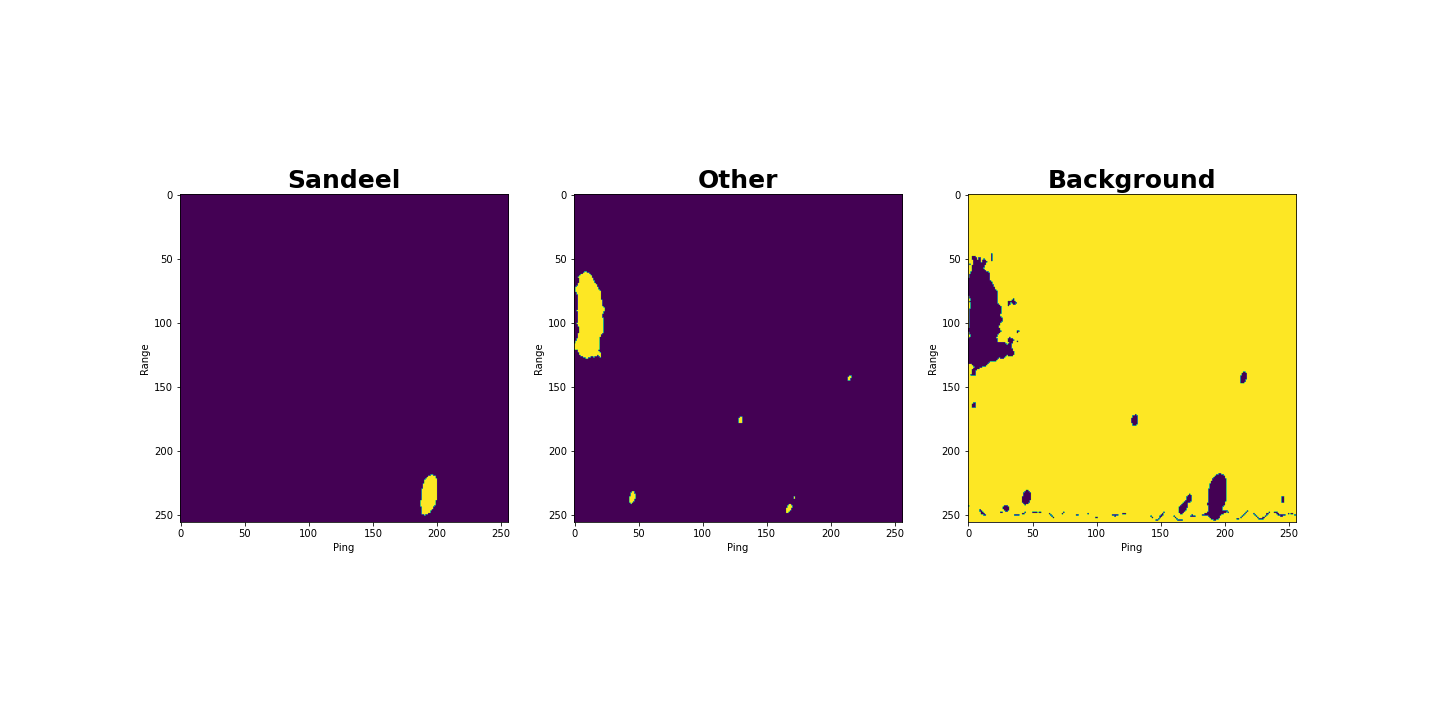
\includegraphics[width=1\textwidth]{figures/data_sample.png} } 
        
        \subfloat[Vertical flipping.]{
        	\includesvg[inkscapelatex=false,width=0.9\textwidth,keepaspectratio]{figures/vertical_flip_clown.svg}}
        
        
        \caption[Two data augmentation examples]{Two augmentation methods applied to the same image.}
        \medskip 
        \hspace*{15pt}\hbox{\scriptsize Credit: Original image (\textit{Both left pictures above}) by Nick Hobgood \cite{clownfish_image}}
        \label{data augmentation fig}
        
        \end{figure}
    

\section{U-Net} \label{unet}

    In this section, we introduce the architecture of the model that is the backbone of the work in this thesis. U-Net is a fully convolutional, state-of-the-art \cite{rajak2021segmentation} semantic segmentation \gls{cnn} initially developed for biomedical image analysis by \citeauthor{unet_ronneberger2015} \cite{unet_ronneberger2015}. 
    
    \begin{figure}[H]
        \centering
        %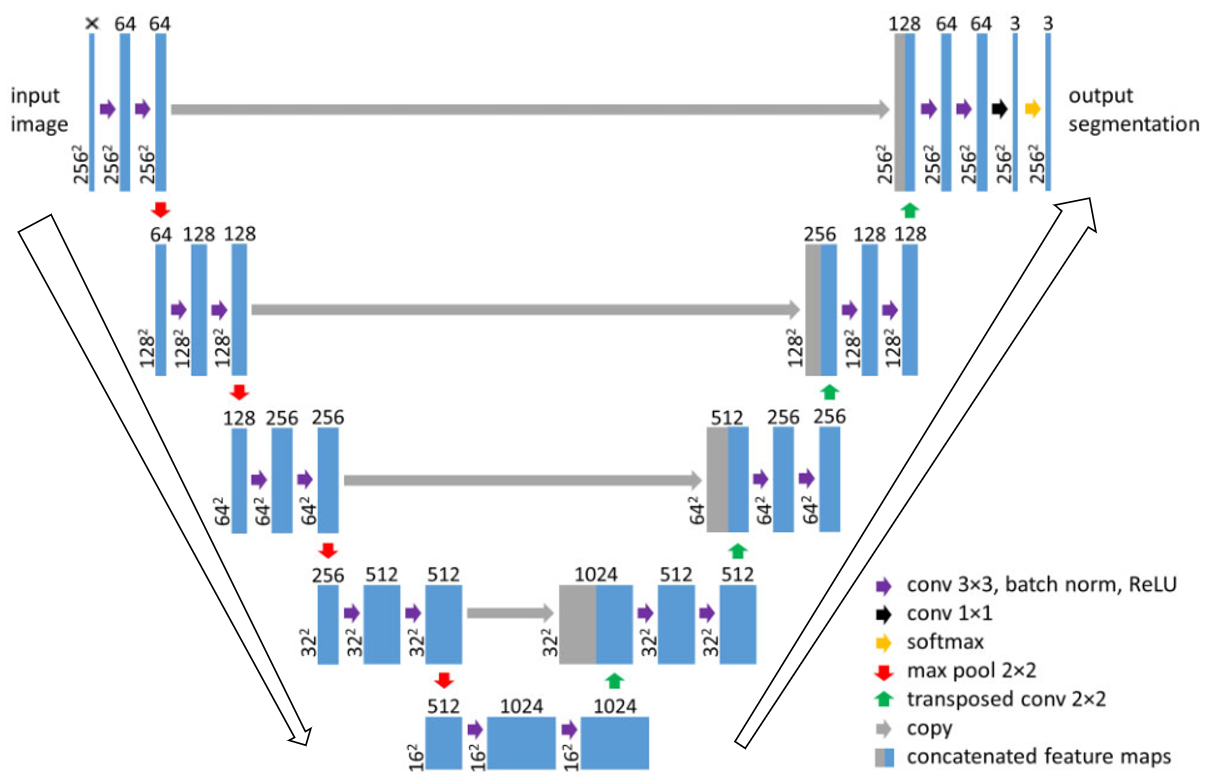
\includegraphics[scale=0.5]{figures/unet_arrows.png}
        \includesvg[inkscapelatex=false,width=1.0\textwidth,keepaspectratio]{figures/unet_original.svg}
        \caption[U-Net architecture]{The U-Net architecture, the downwards facing arrow illustrates the contracting path and the one facing upwards is the expanding path. For each block, the vertical number is the resolution, while the horizontal is the number of feature channels. The color gets darker as the channels increase.}
      	\medskip 
        \label{unet_fig}
        \hspace*{15pt}\hbox{\scriptsize Credit: \citeauthor{unet_ronneberger2015} \cite{unet_ronneberger2015}}
    \end{figure}
    
    %Each stage applied the same operations to its given input.
    
    U-Net utilized what \citeauthor{unet_ronneberger2015} \cite{unet_ronneberger2015} called a \textit{contracting path} to identify what was in a picture, while an \textit{expanding path} localized where it was. These two branches were more or less symmetrical, and together they formed a U-shape, giving the network its name. The contracting path can be looked at as five different stages of processing, from top to bottom, in figure \ref{unet_fig}. Each stage consisted of two 3×3 valid convolutions with their individual ReLU activation functions. Initially, the feature channels are increased to 64, and the channels were doubled for each contracting stage. The convolutions were followed by a 2×2 max pooling operation with stride 2 to further decrease the resolution of the output from the convolutional operations and then output a feature map to the next stage. After the bottom stage, the max pool operation is replaced with transpose convolutions to now increase the resolution. At each subsequent stage traveling back up the expanding path, the number of feature channels is halved by the convolutional steps down to 64. 
    
    In the expanding path, the previous stage's output was concatenated with a crop from the output feature map of a stage from the contracting path with the same channel size, the cropping is due to different resolutions. This step allows the following expanding path convolutional operation to access both the high-resolution feature map from the contracting path and the upsampled feature map, which in combination helps with the localization of features \cite{unet_ronneberger2015}. 

    At the final layer in the expanding path, a 1×1 convolution maps the 64 feature channels to the user defined number of classes, which is two classes in figure \ref{unet_fig}. Finally, the softmax was then calculated between these classes, giving each pixel a probability distribution over the classes, with one channel for each class. Hence, giving us a segmentation map \cite{unet_ronneberger2015}.
    
    %Hence, these layers increase the resolution of the output. In order to localize, high resolution features from the contracting path are combined with the upsampled output. A successive convolution layer can then learn to assemble a more precise output based on this information.
    
    
    When released, U-Net outperformed other networks in multiple biomedical challenges \cite{unet_ronneberger2015}. Its performance inspired new models that use the U-Net architecture as their backbone, as seen in NAS-Unet \cite{weng2019unet} in \citeyear{weng2019unet}, and Unet++ \cite{zhou2018unet} in \citeyear{zhou2018unet}. U-Net has also been applied successfully  to other fields such as road extraction in satellite images by \citeauthor{zhang2018road} \cite{zhang2018road} in \citeyear{zhang2018road}, and on acoustic classification by \citeauthor{brautaset2020acoustic} \cite{brautaset2020acoustic} in \citeyear{brautaset2020acoustic}, which will be explained in the following chapter.
    
    %In the field of biomedicine, data are scarce and so heavy use of data augmentation was applied, which made the U-Net able to train on very few samples.
    
    %At the last stage, a 1×1 convolution was applied instead of increasing the resolution.





